\documentclass[12pt]{report}
\usepackage[a4paper, height=10in, width=8in, hmargin={2cm,0.8in}]{geometry}
\usepackage{graphicx} % Required for inserting images
\usepackage{xeCJK}
\usepackage{amssymb}
\usepackage{amsthm}
\usepackage{amsmath}
\usepackage{caption}
\usepackage{comment}
\usepackage{subcaption}
\usepackage{enumerate}
\usepackage{multirow}
\usepackage{physics}
\usepackage[separate-uncertainty=true]{siunitx}
\usepackage{multirow}
\usepackage{booktabs}
\usepackage{chemformula}
\usepackage{sectsty}
\usepackage{svg}
\usepackage{url}
\usepackage{titlesec}
\usepackage{fontenc}
% \usepackage[width=0.9\textwidth]{caption}

\newcommand{\chapfnt}{\fontsize{18}{20}}
\titleformat{\chapter}[hang]
{\normalfont\chapfnt\bfseries}{\thechapter}{20pt}{\chapfnt}

\setCJKmainfont{NotoSansTC-Regular}
\renewcommand{\baselinestretch}{1.25}

\DeclareMathOperator{\TGC}{TGC}

\title{112-2 近代物理實驗\\Ultrasonic Comprehensive\\\vspace{1cm}
\includegraphics[width=0.5\textwidth]{Group photo}
}
\author{週一班第二組 \\ 左:林馳耘 B10202037 中:吉芸萱 B10202036 右:丁安磊 B10202051}
\date{實驗日期:04/29, 05/06, 05/07/2024\\提交日期: 05/20/2024}

\begin{document}

\renewcommand{\figurename}{圖}
\renewcommand{\tablename}{表}
\newcommand{\br}[1]{\left(#1\right)}
\renewcommand{\vb}[1]{\boldsymbol{\mathbf{#1}}} % New vector bold command to adapt for greek letters.

\maketitle

\tableofcontents

\clearpage

% \begin{figure}[htbp]
%     \centering
%     \begin{subfigure}{0.49\textwidth}
%         \centering
%         \includegraphics[\textwidth]{name}
%         \caption{<caption>}
%         \label{<label>}
%     \end{subfigure}
%     \hfill
%     \begin{subfigure}{0.49\textwidth}
%         \centering
%         \includegraphics[\textwidth]{name}
%         \caption{<caption>}
%         \label{<label>}
%     \end{subfigure}
% \end{figure}

\chapter{引言}

本次實驗為兩週實驗,必做的實驗為PHY04, 05, 06, 07, 11, 23,第一週我們進行了PHY04, 05, 11的實驗,
並初步了解實驗儀器與軟體的操作,並研究了軟體匯出的數據形式。第二週進行了PHY06、PHY07的實驗,
由於進行PHY06的實驗時也嘗試了作PHY01的實驗耽誤到了一些時間,所以沒有將必做的實驗做完,於是在隔天補做了PHY23的實驗。

\section{實驗儀器基本介紹、軟體操作}

超聲波探測儀GS200為本實驗中主要使用的儀器,有兩個探針的接口可以連接,在探測反射回聲時通常使用 Reflection mode(只需連接探針 1,兼負訊號的發射與接收),如PHY01, 04, 05, 06實驗。而在探測透射的聲波時則會連接兩個探針分別用於收發,如PHY07, 23實驗。
GS200連接到電腦上的GS-EchoView程式,我們只會用到其中的A-mode,包含四種圖表:
\begin{enumerate}
\item A-scan: Receiver 探針 接收到的時域訊號。包含原始訊號(HF)以及訊號的振幅(Amp)。
\item Spectrum FFT: 透過選取A-scan中的時間範圍,進行快速傅立葉變換(Fast Fourier Transform, FFT)得到頻域訊號
\item TGC(Time Gain Control): 因為聲波在傳遞的過程中會發生衰減,GS200除了能夠調整收發的Gain和Output大小,還能透過TGC將不同時間的訊號進行放大,使得回聲訊號能被探測到。
\item Cepstrum: 由FFT訊號得到的倒頻譜訊號(見PHY05實驗)。
\end{enumerate}
透過Cursor,我們能在這些圖表上標示出需要的點。然而,為了更精準地測量數據,我們也會將訊號匯出做計算。其中,當A-scan的絕對數值是重要的時候,我們需要紀錄TGC的形式,如PHY04中需要計算訊號的衰減。但如果A-scan僅有相對數值重要時,比如只需計算聲波回聲的起始位置和峰值位置,則不需考慮TGC數值。

% 在記錄數據時,我們發現儀器可以讀取的振幅上限為 1,若超過則波形會成方波,此時數據已失準。因此必須調整 TGC 參數,在上限內使得訊號盡量大。

% 3) 凝膠用量誤差 本實驗中,若凝膠用量過少、或接觸面有氣泡會導致超聲 波傳導不順,影響實驗結果。此外,若凝膠用量過多,接觸面凝膠 的厚度又會使待測物的厚度變大,造成誤差。且每次塗抹凝膠的量 不相同,或使用過的凝膠沒有完全清除乾淨,都會影響實驗結果。

\section{不確定度分析方法}

本次實驗報告使用了 Python 進行數據的讀取與分析,列舉幾個其中主要的 package 與函式如下:
\begin{itemize}
    \item \verb|scipy.stats.linregress|: 用於擬合直線$y=ax+b$,可以得出斜率與截距的最佳估計值、不確定度,以及擬合的$R^2$值。
    \item \verb|uncertainties.ufloat|: 包含最佳估計值與不確定的浮點數值,對其直接進行運算(如加減乘除)可以得到不確定度傳遞的結果。
    \item \verb|uncertainties.unumpy|: 能夠對\verb|ufloat|物件進行函數運算,比如\verb|unumpy.log|,可以獲取帶有不確定度的數值取對數後的最佳估計值以及不確定度,如此便可以簡便地計算廣義不確定度傳遞的結果:
    \begin{equation}
        \sigma_f = \sqrt{\sum_i \left(\frac{\partial f}{\partial x_i}\right)^2 \sigma_{x_i}^2}
    \end{equation}
\end{itemize}

圖\ref{fig:unc}示範了如何使用這些 package 進行不確定度分析。

\begin{figure}[htbp]
    \centering
    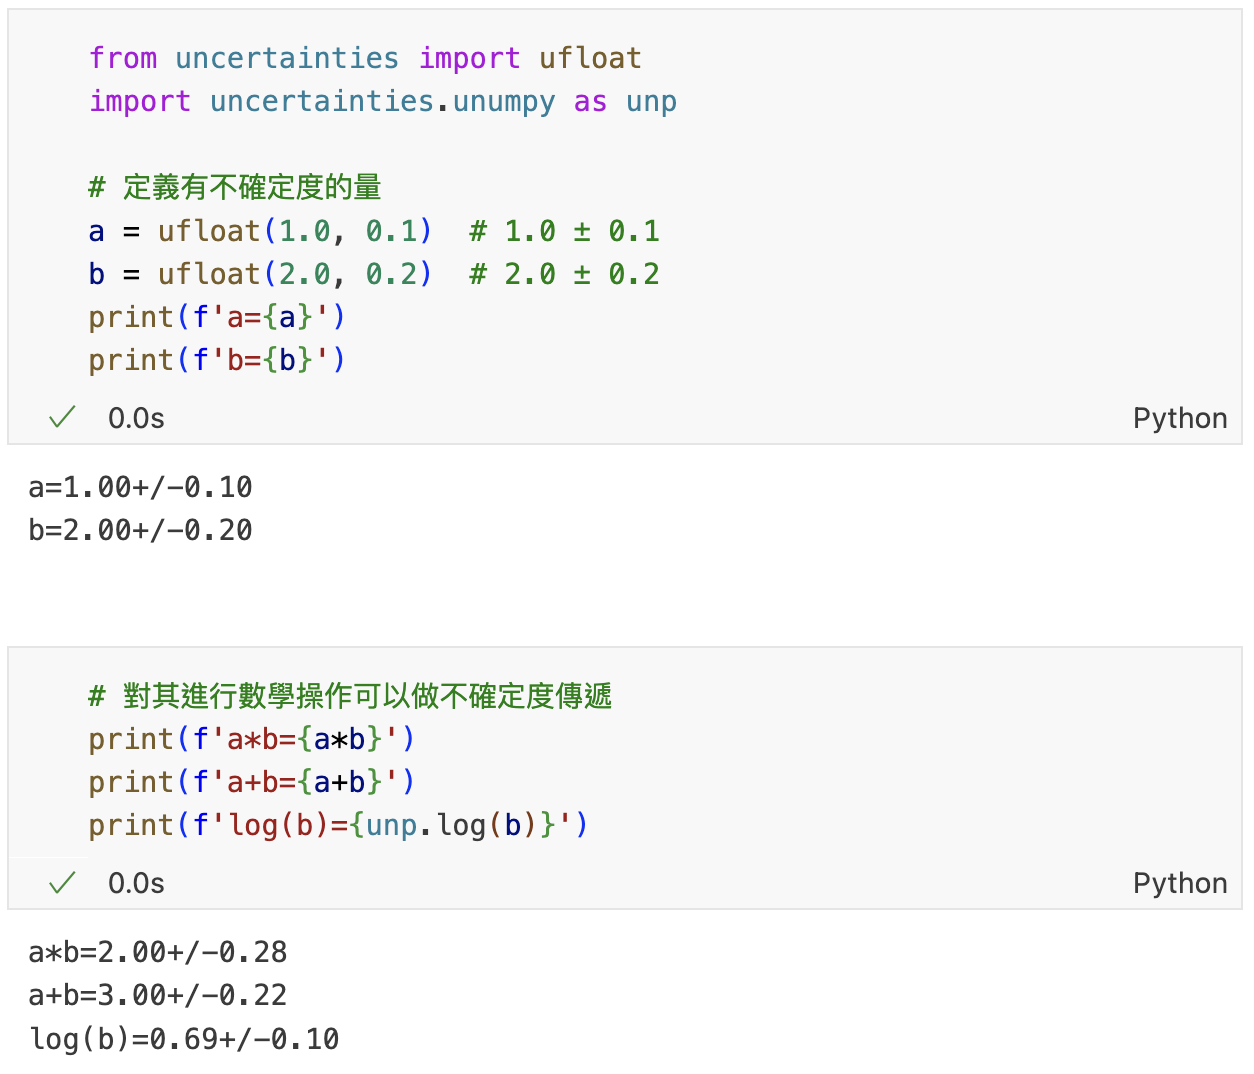
\includegraphics[width=0.5\textwidth]{unc.png}
    \caption{不確定度分析示範}
    \label{fig:unc}
\end{figure}

\chapter{PHY04 Attenuation of ultrasound in liquids}\label{PHY04}

\section{實驗目的}
求得\SI{1}{MHz}超聲波在水中的衰減係數(attenuation coefficient) $\alpha$

\section{實驗原理}

\subsection{對數單位}

在計算物理量的水平(Level)的時候我們會區分場量(field quantity)和功率量(power quantity)的概念。在聲學中,場量即為聲壓,其正比於我們在儀器上測量到的電壓振幅$A$,場量的平方值在一個線性系統中與功率成比例。而功率量是聲音強度$I$,與聲波的功率值成比例。振幅$A$相較於基準值$A_0$的水平在不同對數單位下的定義為
\begin{equation}
    L_A = \ln\left(\frac{A}{A_0}\right)[{\rm Np}] = 2\log_{10} \left(\frac{A}{A_0}\right) [{\rm B}] = 20\log_{10} \left(\frac{A}{A_0}\right) [{\rm dB}]
\end{equation}
從這裡我們可以看出$\SI{1}{Np}=20\log_{10}(e)\ \si{dB}\approx \SI{8.686}{dB}$,上述公式可改寫成
\begin{equation}
    A = A_0\times e^{L_A\ [{\rm Np}]} = A_0\times 10^{L_A\ [{\rm dB}]/20}
\end{equation}

\subsection{聲波在液體中的衰減}
當聲波在液體中傳播時,由於吸收(能量轉換)、反射、散射或聲場的幾何形狀而衰減。在水中,低頻吸收、反射和散射可以忽略不計。所以我們只需要考慮聲場幾何形狀導致的衰減,聲波強度的衰減可以描述為
\begin{equation}
    I=I_0 e^{-\alpha x}
\end{equation}
其中$I_0$為初始強度,$x$為聲音在液體中行經的路徑長,$\alpha$為衰減係數。因為$I\propto A^2$,我們有
\begin{equation}
-2\ln\left(\frac{A}{A_0}\right) [{\rm Np}] = \alpha x
\end{equation}
依照前述的方法進行單位換算
\begin{equation}\label{eqn:attenuation}
-2\times 8.686 \times \ln\left(\frac{A}{A_0}\right) [{\rm dB}] = \alpha x
\end{equation}
因此我們可以進行多次不同路徑長及對應衰減後振幅的測量來求得$\alpha$。在講義中,會選取第一次測量結果作為基準值並進行線性回歸,
但我們認為這樣會依賴於第一次測量的準確性。事實上,我們可以直接測量所有振幅值(相對於基準值\SI{1}{V})的對數值$\ln\left(\frac{A}{\SI{1}{V}}\right)$,並與$x$進行線性回歸得到斜率,即可求出$\alpha$。

\section{實驗步驟}

\begin{enumerate}
    \item 將儀器架設如圖\ref{fig:PHY04_apparatus},水槽及 探針 的交界要用 ultrasonic gel 連接,將 探針 調整為 Reflection mode。
    \item 移動鋁板的位置並記錄其位置,並匯出A-scan的波形。
    
    在這裡我們選擇紀錄的距離為其上方的黑色塑膠邊緣到容器壁的距離$d$。不用直接測量鋁板的容器壁的原因是,由A-scan的波形我們可以得知回聲發生的時間$t_{\rm echo}$,將$d$與$t_{\rm echo}$進行線性回歸,其負截距即為我們少測量到的黑色塑膠邊緣到鋁板的距離$d_0$。注意到,由於聲波在鋁板反射才被 探針 接收,聲波在水中行經的路徑長應為$x=2(d+d_0)$。

    \item 需注意這些不同位置的測量要保持同樣的 Output、Gain和TGC形式,最終匯出TGC的波形。
    
    注意到Output和Gain會同時放大所有測量的振幅,所以影響可以忽略不計。但是TGC會隨著測量距離不同而對振幅進行不同程度的放大,
所以需要紀錄其波形並在數據分析時考量其影響。

\begin{figure}[htbp]
    \centering
    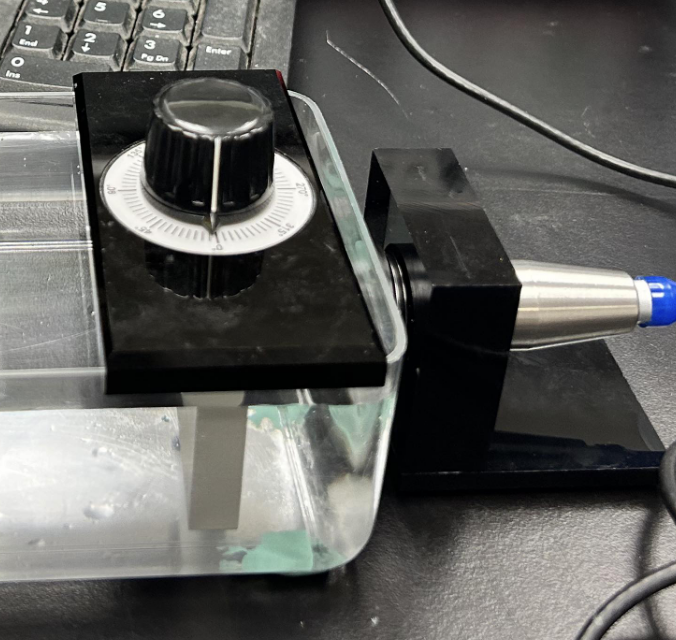
\includegraphics[width=0.5\textwidth]{PHY04_appratus.png}
    \caption{PHY04儀器實拍圖}
    \label{fig:PHY04_apparatus}
\end{figure}

\end{enumerate}

\section{結果與討論}

\subsection{TGC數據}

TGC的參數包含Threshold、Wide、Slope、Start,會在一段時間範圍對振幅進行放大,其放大程度與時間成線性關係。對TGC數據的線性範圍進行擬和,
可以得到$\TGC(t)=(0.077\times t\ [\si{\micro\second}] - 0.57) \ [{\rm dB}]$,如圖\ref{fig:phy04_tgc}。

\begin{figure}[htbp]
    \centering
    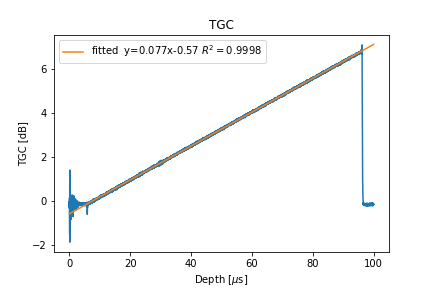
\includegraphics[width=0.5\textwidth]{PHY04_TGC.png}
    \caption{TGC及其線性範圍內的擬合}
    \label{fig:phy04_tgc}
\end{figure}

\subsection{校正鋁板位置}

回聲的波形如圖\ref{fig:phy04_ascan},首先說明如何求得$t_{\rm echo}$:設定一個大於噪聲的閾值,並找出第一個Amp大於該閾值的時間點,即為$t_{\rm echo}$。將測量的距離$d$對$t_{\rm echo}$進行擬和,如圖\ref{fig:phy04_speed},其斜率值的兩倍即為水中聲速$c_0=\SI{1481.6(15)}{m/s}$,與當時溫度\SI{20}{\celsius}下水的聲速的公認值\SI{1482}{m/s}吻合。其截距的負值為$d=\SI{2.103(8)}{cm}$。校正後的鋁板位置即為$d+d_0$,且聲波的衰減深度為$x=2(d+d_0)$。

\begin{figure}[h]
    \centering
    \begin{subfigure}{0.49\textwidth}
        \centering
        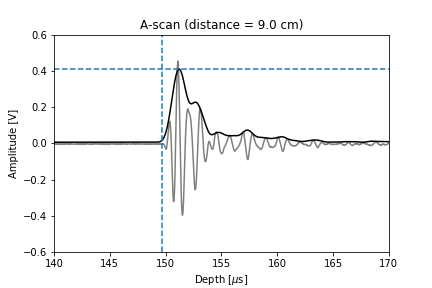
\includegraphics[width=\textwidth]{PHY04_ascan.png}
        \caption{回聲波形,其中水平虛線表示Amp值的最大值$A'$,垂直虛線表示回聲的起始時間}
        \label{fig:phy04_ascan}
    \end{subfigure}
    \hfill
    \begin{subfigure}{0.49\textwidth}
        \centering
        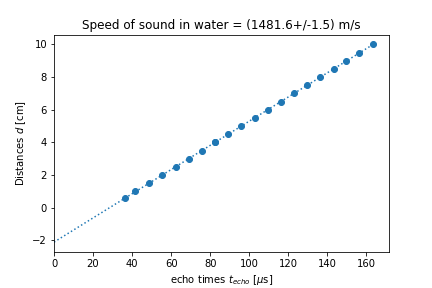
\includegraphics[width=\textwidth]{PHY04_speed.png}
        \caption{測量的距離與回聲起始時間的關係圖}
        \label{fig:phy04_speed}
    \end{subfigure}
    \caption{校正鋁板位置}
\end{figure}

\subsection{計算衰減係數}

在回聲的範圍內尋找Amp值的最大值$A'$及其峰值時間$t_{\rm peak}$,如圖\ref{fig:phy04_ascan}。設回聲的實際大小為$A$,由於TGC的放大所以有
\begin{equation}
    A'=A\times 10^{\TGC(t_{\rm peak})[{\rm dB}]/20}
\end{equation}
考量TGC的影響求出$A$。改寫\ref{eqn:attenuation}成
\begin{equation}\label{04fit}
    -2\times 8.686 \times \ln\left(\frac{A}{\SI{1}{V}}\right)= \alpha x -2\times 8.686 \times \ln\left(\frac{A_0}{\SI{1}{V}}\right)
\end{equation}
計算$-2\times 8.686 \times \ln\left(\frac{A}{\SI{1}{V}}\right)$,對$x$進行線性回歸,如圖\ref{fig:phy04_result},可發現結果的確是線性的,得到的斜率即為$\alpha=\SI{1.493(32)}{dB/cm}$。

水的衰減係數與頻率成線性關係(我們僅有使用\SI{1}{MHz}進行測量),理論值為$\alpha/f=\SI{0.0022}{dB/cm/MHz}$。可以發現我們的測量值遠大於理論值。由於我們已經透過程式分析排除了讀取Cursor產生的誤差,也綜合考量的TGC的影響(若沒有考量TGC的影響會發現並非線性關係,如圖\ref{notgc}),我們嘗試分析幾個誤差的來源:
\begin{itemize}
    \item 水槽的幾何形狀造成的 damping 比我們預期的多:由於理論中聲波的衰減是由於聲波的能量在空間中平均分佈於立體角,而水槽中有限的空間可能會對衰減的現象產生影響。
    \item 前面提到聲波的衰減現象由很多的因素組成,我們使用的水中可能有雜質使得散射現象也造成了衰減。
    \item 鋁板並不是一個很好的反射板,且探針經過容器壁的壓克力也會發生部分的吸收:鋁板的水中的反射率僅為
    \begin{equation}
        R=\left(\frac{c_2\rho_2-c_1\rho_1}{c_2\rho_2+c_1\rho_1}\right)^2=0.641
    \end{equation}
    其中水中和鋁板中聲速分別為$c_1=\SI{1490}{m/s}$, $c_2=\SI{5000}{m/s}$。密度分別為$\rho_1=\SI{1000}{kg/m^3}$, $\rho_2=\SI{2700}{kg/m^3}$。直覺上來看鋁板的部分反射將會使得衰減係數產生正偏差。但事實上因為每筆數據點都受到了一樣的衰減,
    這就有如我們調整GAIN和OUTPUT旋鈕一樣。從式\eqref{04fit}的角度來說,總體的衰減只會影響擬合的截距而不會影響斜率$\alpha$,同樣的道理,聲波在探針、容器壁、水之間的介面發生的透射造成的影響也可以被排除。
\end{itemize}

\begin{figure}[htbp]
    \centering
    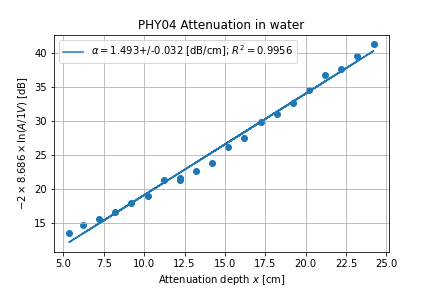
\includegraphics[width=0.5\textwidth]{PHY04_result.png}
    \caption{$-2\times 8.686 \times \ln\left(\frac{A}{\SI{1}{V}}\right)$對$x$進行線性回歸的結果}
    \label{fig:phy04_result}
\end{figure}

\begin{figure}[htbp]
    \centering
    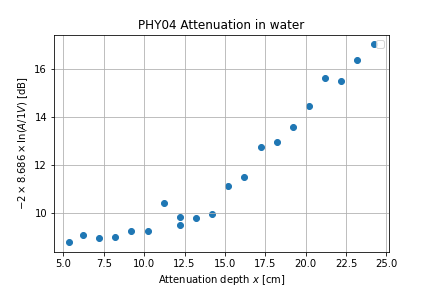
\includegraphics[width=0.5\textwidth]{noTGC.png}
    \caption{$-2\times 8.686 \times \ln\left(\frac{A'}{\SI{1}{V}}\right)$對$x$關係,沒有考慮TGC影響}
    \label{notgc}
\end{figure}

\chapter{PHY05 Spectral investigations}\label{PHY05}

\section{實驗目的}

將超聲波在三種長方體薄板中經過多次反射的訊號利用快速傅立葉變化(Fast Fourier Transformation, FFT)進行頻譜分析;再進一步將 FFT 後的頻譜 (Spectral) 進行變換為倒頻譜(Cepstrum),並以 Cepstrum 上之週期得出薄板厚度,並與其他方法得到的厚度做比較。

\section{實驗原理}

\subsection{快速傅立葉變換}

快速傅立葉變換(Fast Fourier Transformation; FFT)為離散時間傅立葉變換(Discrete Time Fourier Transformation; DFT)之推廣,DFT能將離散時間測得的訊號藉由傅立葉矩陣(Fourier Matrix)從時域轉到頻域以利訊號分析的
進行,也能夠透過其逆變換IFFT從頻域轉換到時域,實驗的軟體有內建FFT的功能,我們也可以將匯出的A-scan透過\verb|scipy.fftpack|的套件進行FFT與IFFT,為了驗證程式碼的正確性,我們有將程式得到的FFT結果與軟體得到的結果進行比較。

\subsection{倒頻譜}

計算倒頻譜(Cepstrum)需要三個步驟:
\begin{enumerate}
    \item 將訊號使用FFT由時域轉為頻域。
    \item 將頻域的振幅大小取對數
    \item 將取過對數的資料進行IFFT轉回時域,即為倒頻譜
\end{enumerate}
倒頻譜可以視為頻譜中不同頻率的變化,能用來量測回聲之間的間隔時間。

\section{實驗步驟}

\begin{enumerate}
\item 用游標尺測量三個薄板的厚度
\item 將壓克力圓柱與薄板以超聲波膠連結。
\item GS200 以 Reflection mode 設定,連結\SI{2}{MHz} 探針。
\item 調整 Gain 與 Output,調整 TGC。
\item A-scan選取數個回聲訊號的時間範圍進行FFT,得到對應的Cepstrum。
\item 匯出A-scan、Spectrum FFT、Cepstrum的波形。
\end{enumerate}

超聲波從圓柱頂端打入傳遞到薄板位置發生反射與透射,反射的訊號被接收行程第一個回聲訊號,而透射的訊號穿越薄板並反射,而形成第二個回聲訊號。不斷反射與透射將產生數個回聲訊號,每個訊號之間約有$\Delta t = 2d/v$的延遲,其中$d$為薄板厚度,$v=\SI{2670}{m/s}$為該薄板中的聲速。

為了得到這個延遲時間的大小並求得薄板厚度,我們有三種方法:

\subsection{方法一:使用Ascan中的峰值時間}

第一種最直覺的方法就是直接分析回聲訊號中的峰值位置並計算差距得到這個延遲。以薄板2為例,
在回聲的範圍中尋找Ascan中Amp最大的位置,如圖\ref{fig:05a}所示。

\subsection{方法二:使用多個回聲訊號的FFT峰與峰之間的頻率差計算}

同樣以薄板2為例,當我們對其中一個回聲訊號進行FFT,只會得到一個峰值,對應到探針發射的頻率。但如果我們選取方法一中的時間範圍進行FFT,這三個回聲訊號可以視為是週期更大的訊號,基頻為$F_0$,將會在FFT中基頻的倍數處產生峰值,如圖\ref{fig:05f}所示。計算這些峰值之間的頻率差的平均值即為$F_0$,取倒數$T_0=1/F_0$即為薄板中的飛行時間。注意到FFT有幾個峰並不是完全尖的,這會使得對於基頻的估計有偏差。

% \begin{figure}[htbp]
%     \centering
%     \begin{subfigure}{0.49\textwidth}
%         \centering
%         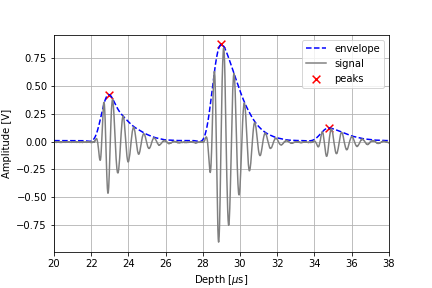
\includegraphics[width=\textwidth]{PHY05_ascan.png}
%         \caption{方法一:使用Ascan中的峰值時間}
%         \label{fig:05a}
%     \end{subfigure}
%     \hfill
%     \begin{subfigure}{0.49\textwidth}
%         \centering
%         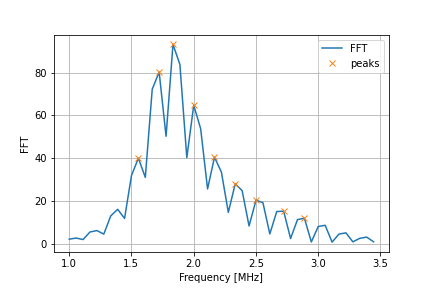
\includegraphics[width=\textwidth]{PHY05_fft.png}
%         \caption{方法二:使用多個回聲訊號的FFT峰與峰之間的頻率差計算}
%         \label{fig:05f}
%     \end{subfigure}
% \end{figure}

\begin{figure}[h]
    \centering
    \begin{subfigure}{0.49\textwidth}
        \centering
        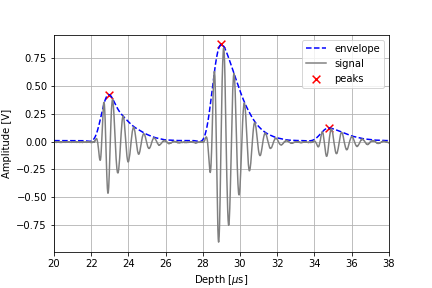
\includegraphics[width=\textwidth]{PHY05_ascan.png}
        \caption{方法一:使用Ascan中的峰值時間}
        \label{fig:05a}
    \end{subfigure}
    \hfill
    \begin{subfigure}{0.49\textwidth}
        \centering
        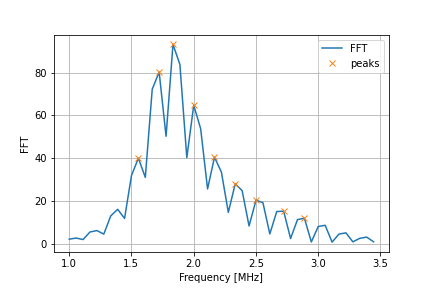
\includegraphics[width=\textwidth]{PHY05_fft.png}
        \caption{方法二:使用多個回聲訊號的FFT峰與峰之間的頻率差計算}
        \label{fig:05f}
    \end{subfigure}
    \caption{計算回聲間距的前兩種方式}
\end{figure}

\subsection{方法三:使用倒頻譜}

利用倒頻譜對頻譜進行平滑處理,可以在倒頻譜的時間軸上分離出等距離的頻率間隔,如圖\ref{fig:05c},使用倒頻譜能清楚地得到我們的時間差$\Delta t$,並加以獲得薄板的厚度$d$。由上述資料我們可以發現,使用 Cepstrum 法測得的數據最準確。由於 Cepstrum 法能夠以對數函數保留、強調 FFT 圖中間隔為$F_0$ 之波峰,由此逆推 FFT 圖形的譜線,將會比原始飛行時間的圖片有更好之解析度,我們也能得到更準確的結果。

\begin{figure}[htbp]
    \centering
    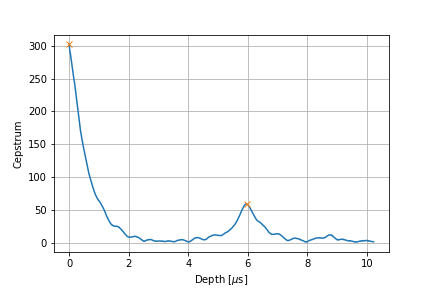
\includegraphics[width=0.5\textwidth]{PHY05_ceps.png}
    \caption{方法三:使用倒頻譜計算回聲間距}
    \label{fig:05c}
\end{figure}

\section{結果與討論}

整理三種方法測得的薄板厚度如表\ref{tab:phy05},可以發現倒頻譜得到的結果最為準確。但還是沒有落在不確定度範圍內。推測原因為講義中聲速的理論值的偏差導致,假設聲速有0.6\%的相對不確定度,即$v=\SI{2670(16)}{m/s}$,那麼游標尺和倒頻譜的測量結果將會吻合(即有重疊的不確定度範圍)。

\begin{table}[htbp]
    \centering
    \caption{三個薄板的測量厚度,與分別使用三種方法測量得到的厚度。(單位:cm)}
    \label{tab:phy05}
    \begin{tabular}{@{}cccccccc@{}}
    \toprule
    薄板 & 測量厚度           & A-scan & error  & Spectrum & error & Cepstrum & error  \\ \midrule
    1  & \SI{8.90(1)}{} & 9.05   & 1.7\%  & 9.01     & 1.2\% & 8.95     & 0.6\%  \\
    2  & \SI{7.96(1)}{} & 7.90   & -0.7\% & 8.01     & 0.6\% & 7.96     & -0.0\% \\
    3  & \SI{5.80(1)}{} & 5.76   & -0.7\% & 6.00     & 3.5\% & 5.82     & 0.4\%  \\ \bottomrule
    \end{tabular}
\end{table}





















\chapter{PHY06 Frequency dependence of resolution power}\label{PHY06}

\section{實驗目的}
探討不同頻率的超聲波的軸向分辨率,研究其是否能分辨出Acrylic test block上兩個距離相近的小洞,並計算他們對不同的大洞的反射脈衝的寬度。

\section{實驗原理}

不同頻率的探針產生的聲波脈衝寬度不同,隨著頻率的增加,聲脈衝變短,其在軸向上分辨率提高,但穿透的深度會隨著頻率的
增加而減小。我們定義脈衝寬度(Pulse Width)為聲波振幅的半高寬(Full Width at Half Maximum; FWHM),根據講義,理論上脈衝寬度為聲波波長的兩倍:
\begin{equation}
    \frac{c\Delta t}{\lambda} = \frac{\Delta t}{T} = 2
\end{equation}
其中$\Delta t$為時域上的脈衝寬度。

\section{實驗步驟}

\begin{enumerate}
    \item 使用游標尺測量Test Block的長寬高。
    \item 將探針的模式調整為Reflection mode。
    \item 使用探針測量Test Block的邊界造成的回聲,調整探針的位置使得反射的路徑盡量不要經過其中的洞造成多餘的反射。對三個邊都進行測量。
    \item 選取Test Block中的不同的大洞,紀錄各個探針對這些洞反射的脈衝的A-scan檔案。
    \item 將探針對準其中兩個相鄰的小洞,紀錄兩個小洞反射產生的脈衝的A-scan檔案。
\end{enumerate}

\section{結果與討論}

\subsection{Test Block的尺寸測量與聲速計算}

游標尺最小單位\SI{0.02}{mm},因此B類不確定度為$\SI{0.02}{mm}/\sqrt{3}=\SI{0.01}{mm}$,測量Test Block的三個維度分別為:
\begin{equation}
    x_1=\SI{42.00(1)}{mm},\quad x_2=\SI{80.46(1)}{mm},\quad x_3=\SI{150.44(1)}{mm}    
\end{equation}
使用三個探針測量Block的三個維度,並使用PHY04中的方法找出由於邊界反射的第一個脈衝的起始位置,如圖\ref{fig:06d},其中由於\SI{4}{MHz} 探針的頻率較高,在Block內將會很快衰減,所以無法找到對於Block的最長邊的反射脈衝。對於每個維度都可以計算聲速為$c=2x/t$,將三個維度計算的聲速取平均即為我們測得之Test Block的聲速,如表\ref{tab:phy06_dim}。

注意到聲波的實際頻率並非探針所標示的1,2,4\ \si{MHz},所以我們要使用FFT讀出聲波的實際頻率$f$,我們選取最短邊造成的反射脈衝進行測量,FFT的範圍標示於圖內。但我們發現,實際上FFT的峰值位置非常依賴於我們FFT選取的範圍,
更好的方法應該是直接觀察A-scan中的波峰位置並直接計算週期(見\ref{sec:pulse_width}脈衝寬度計算)。

\begin{table}[htbp]
    \centering
    \caption{Test Block的聲速\SI{2741.4(20)}{m/s}為三個寬度的回聲測量得到的聲速之平均值。}
    \label{tab:phy06_dim}
    \begin{tabular}{@{}llll@{}}
    \toprule
      & 回聲時間$t$ ($\mu$s)  &  寬度$x$ (mm)  & 聲速$c=2x/t$ (m/s) \\ \midrule
    1 & \SI{30.66(4)}{} & \SI{42.00(1)}{}                & \SI{2740(4)}{}            \\
    2 & \SI{58.64(10)}{}     & \SI{80.46(1)}{}                & \SI{2744(4)}{}               \\
    3 & \SI{109.80(6)}{}     & \SI{150.44(1)}{}                & \SI{2740.3(15)}{}              \\ \bottomrule
    \end{tabular}
\end{table}

\begin{figure}[htbp]
    \centering
    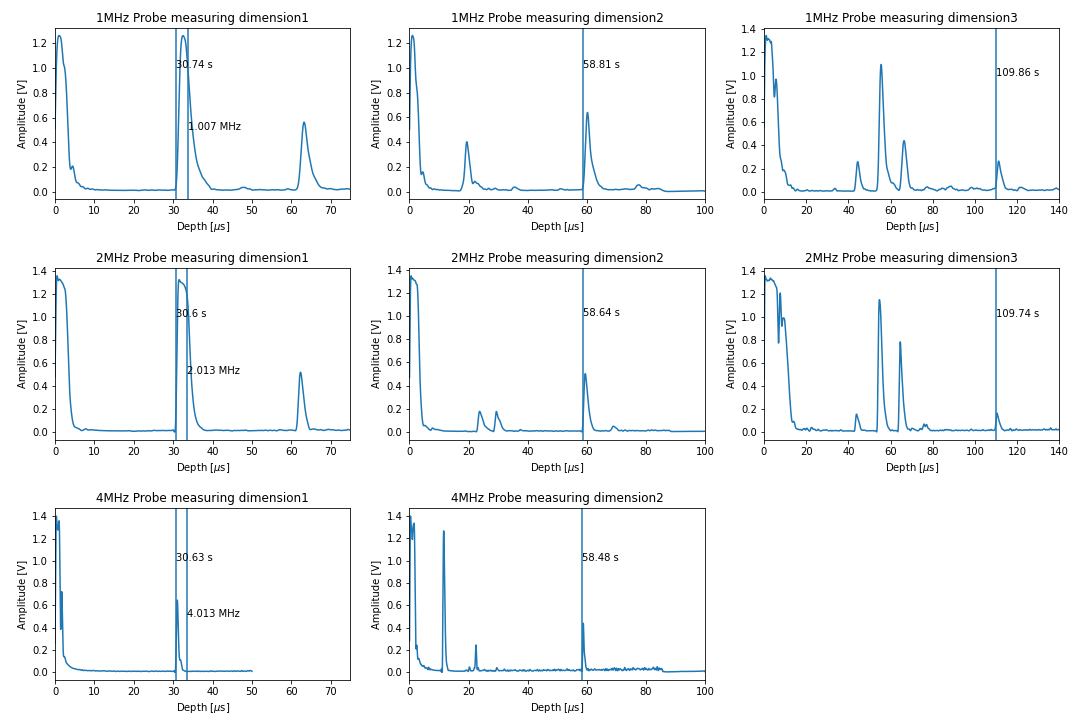
\includegraphics[width=\textwidth]{PHY06_dimensions.png}
    \caption{對Test Block的三個維度的回聲測量,其中4 MHz 探針無法找到dimension 3的回聲。垂直線標示的是第一次回聲發生的起始時間,標示於圖上,在其倍數的位置的訊號對應到多次反射產生的回聲,其他位置的訊號則為Test Block中小孔的反射造成。在Dimension 1中兩垂直線之間表示FFT的範圍,其峰值頻率標示於圖上。}
    \label{fig:06d}
\end{figure}

\subsection{最小可解析距離與小洞間距測量}

使用游標尺可以測量兩個小洞的間距為\SI{1.74}{mm},將此數值視為標準值。使用不同頻率的探針得到的兩小洞的回聲如圖\ref{fig:06r}。
可以發現\SI{1}{MHz}的探針無法分辨出兩個小洞的回聲。而對於更高頻率的兩個 探針,我們有兩種方法分析兩個回聲的間距
\footnote{應該也能使用PHY05的Cepstrum得出兩個回聲的間隔,但是我們當初沒有存到Cepstrum的數據,
也沒有找出使用程式由A-scan結果計算Cepstrum的方法。},
第一種方法是使用兩個回聲的起始時間的間隔計算,第二種方法是使用兩個回聲的峰值時間的間隔計算,使用這兩種方法計算的孔洞間距
如表\ref{tab:phy06_res}。可以注意使用4 MHz的探針測量的誤差較低,且由於兩個回聲完全分離,使用兩種方法得出的結果更一致。

\begin{table}[htbp]
    \centering
    \caption{使用不同頻率的探針與不同方式進行孔洞間距的測量。}
    \label{tab:phy06_res}
    \begin{tabular}{@{}lllrllr@{}}
    \toprule
    頻率 & 起始間隔                   & 孔洞間距   & 誤差    & 峰值間隔                   & 孔洞間距   & 誤差    \\ \midrule
    2MHz & \SI{1.31}{\micro\second} & \SI{1.796(2)}{mm} & \SI{3.9}{\percent} & \SI{1.82}{\micro\second} & \SI{2.495(2)}{mm} & \SI{44.3}{\percent} \\
    4MHz & \SI{1.24}{\micro\second} & \SI{1.711(2)}{mm} & \SI{-1.7}{\percent} & \SI{1.24}{\micro\second} & \SI{1.712(2)}{mm} & \SI{-1.7}{\percent} \\ \bottomrule
    \end{tabular}
\end{table}

\begin{figure}[htbp]
    \centering
    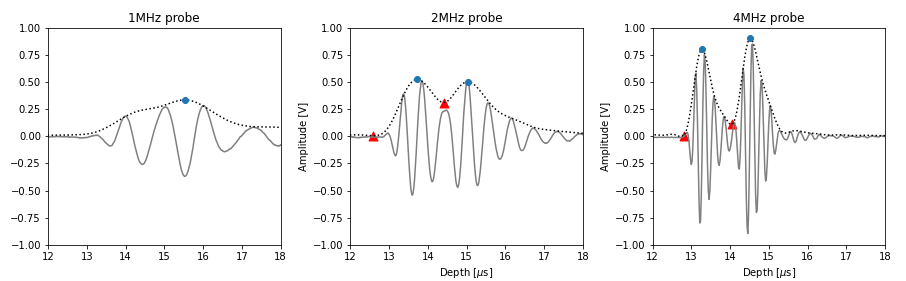
\includegraphics[width=\textwidth]{PHY06_resolution.png}
    \caption{不同頻率的探針的對於小孔的解析:可以發現1 MHz探針測得的兩個回聲完全混合。而更高頻率的探針可以分離兩個回聲,圖中的圓點即為回聲峰值的時間,三角形點則為回聲起始的時間。}
    \label{fig:06r}
\end{figure}

\subsection{脈衝寬度計算}\label{sec:pulse_width}

如圖\ref{fig:06p},使用不同頻率探針,選取幾個洞進行反射,在回聲的範圍內尋找Amp的最大值,找出Amp在其半高以上的範圍,
其寬度即為時域上的脈衝寬度$\Delta t$。在脈衝寬度的範圍內尋找峰值的位置,其間距即為聲波的週期$T$,並計算$\Delta t/T$的值。由於完全使用A-scan的讀取資料進行計算所以沒有進行不確定度的計算,由於我們將資料匯出計算所以可以排除
使用Cursor讀取造成的誤差。比值$\Delta t/T$相對於其理論值$2$產生偏差的主要原因應該是由於色散,導致脈衝波形在材料中行進時發生改變造成。其中低頻1 MHz回聲也因為衰減與色散較少等原因而有比較準確的比值。

\begin{figure}[htbp]
    \centering
    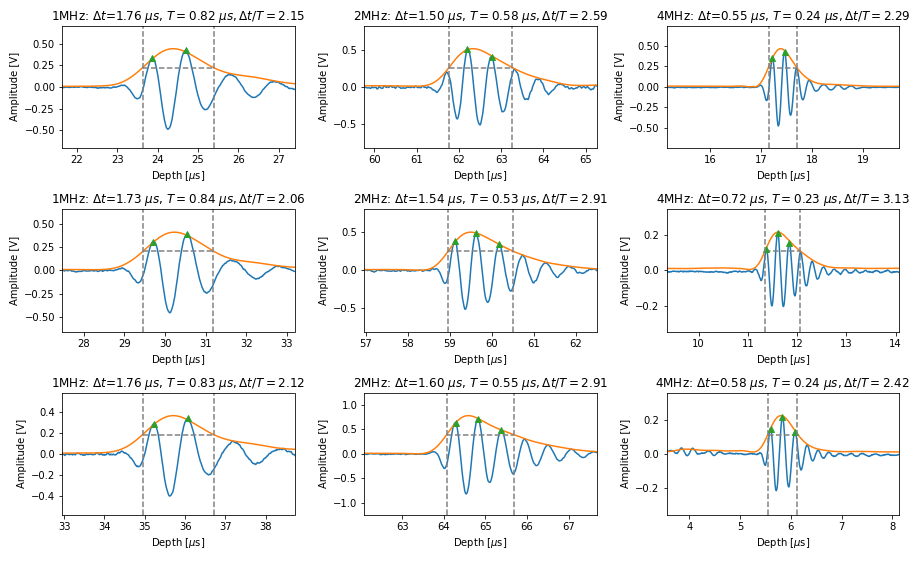
\includegraphics[width=1\linewidth]{PHY06_pulse_width.png}
    \caption{不同頻率探針之脈衝寬度與週期的計算,每個頻率我們各探討三個回聲的訊號。虛線表示FWHM的範圍與高度,其寬度即為脈衝寬度$\Delta t$,三角形點表示訊號的峰值位置,用於計算週期$T$。這些數值與其比值$\Delta t/T$標示於每個子圖的上方。}
    \label{fig:06p}
\end{figure}


\chapter{PHY07 Shear Waves In Solids}\label{PHY07}

\section{實驗目的}
本實驗的目的是研究超聲波之橫、縱波,在浸沒於水中的壓克力板與鋁板中的透射。
並確定這些透射與入射角之間的關係,並計算橫波與縱波分量的聲速。根據材料的彈性係數與其聲速的關係,可以確定彈性係數的大小。

\section{實驗原理}

\subsection{聲波方程與聲波的橫縱波分量}\label{sec:wave_eqn}

將質點的位移$\vb{u}=(u,v,w)$ 透過Helmholtz 分解寫成
\begin{equation}
    \vb u=\nabla\phi+\nabla\times\vb\psi;\quad \nabla\vb\psi=0
\end{equation}
代入彈性材料中的運動方程
\begin{equation}
    \mu \nabla^2 \vb{u} + (\lambda+\mu)\nabla\nabla\cdot \vb{u}=\rho \ddot{\vb{u}}
\end{equation}
其中$\lambda$和$\mu$為Lamé constants,$\rho$為材料的密度。可以得到
\begin{equation}
    \nabla\left[(\lambda+2\mu)\nabla^2\phi-\rho\ddot{\phi}\right]
    +\nabla\times\left[\mu\nabla^2\vb\psi-\rho\vb{\ddot{\vb{\psi}}}\right]=0
\end{equation}
令括號的部分為零,即可得到橫波與縱波的波方程及其波速。
\begin{align}
    \nabla^2\phi-\frac{1}{c_L^2}\ddot{\phi}&=0,\quad c_L^2=\frac{\lambda+2\mu}{\rho} \\
    \nabla^2\vb{\psi}-\frac{1}{c_T^2}\ddot{\vb{\psi}}&=0,\quad c_T^2=\frac{\mu}{\rho}
\end{align}
可以發現縱波的波速大於橫波。

\subsection{聲波斜入射產生的反射與透射}

\begin{figure}[htbp]
    \centering
    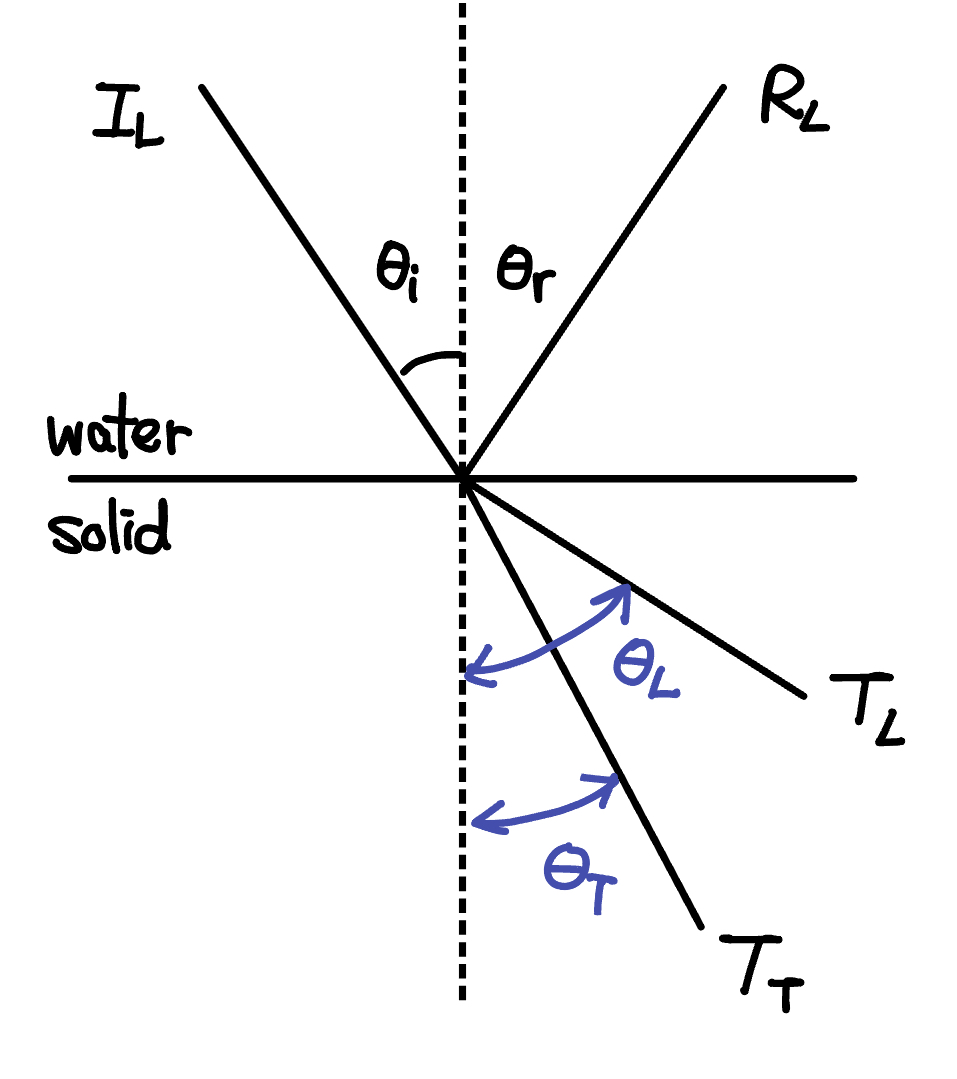
\includegraphics[width=0.5\textwidth]{f2s.jpeg}
    \caption{水中聲波斜向入射固體產生的反射與透射}
    \label{phy07}
\end{figure}

當水中的聲波(縱波)垂直入射固體材料時,僅會產生透射的縱波,如圖\ref{phy07}。但是當縱波以一個入射角$\theta$射入材料時,材料中會產生橫波與縱波的兩分量。若縱波與橫波分別在$\theta=\phi_L$與$\theta=\phi_T$發生全反射,由Snell's law可計算出兩種波在材料中的聲速
\begin{equation}
    c_L = \frac{c_0}{\sin\phi_L};\quad c_T = \frac{c_0}{\sin\phi_T}
\end{equation}
其中$c_0$為水中的聲速。

另外,當橫波的折射波有最大強度時,在固體中的折射角為$\beta=\SI{45}{\degree}$,假設這時的入射角為$\Phi$,則有
\begin{equation}
    \frac{\sin{\Phi}}{c_0} = \frac{\sin{\SI{45}{\degree}}}{c_T}
\end{equation}
所以
\begin{equation}
    c_T = \frac{1}{\sqrt{2}\sin\Phi}c_0
\end{equation}
這提供了另一個求得$c_T$的方法。

\subsection{材料的彈性係數}
Lamé常數和材料中的Elasticity modulus $G$、Shear modulus $G$和Poisson ratio $\nu$的關係為
\begin{equation}
    \mu=G=\frac{E}{2(1+\nu)}
\end{equation}
\begin{equation}
    \lambda = \frac{E\nu}{(1+\nu)(1-2\nu)}
\end{equation}
因此可以將橫縱波的聲速公式改寫為
\begin{equation}\label{speed1}
    c_T = \sqrt{\frac{G}{\rho}}
\end{equation}
\begin{equation}\label{speed2}
    c_L = \sqrt{\frac{E(1-\nu)}{\rho(1+\nu)(1-2\nu)}}
\end{equation}
他們的比值為,
\begin{equation}\label{speed_ratio}
    \frac{c_L}{c_T}=\sqrt{\frac{2(1-\nu)}{1-2\nu}}
\end{equation}


\section{實驗步驟與觀察紀錄}

\begin{enumerate}
    \item 如圖\ref{fig:phy07app}架設器材
    \item 將探針模式調整為 Transmission mode。
    \item 調整材料板的角度,每隔\SI{2.5}{\degree}紀錄一次角度。由於縱波的波速較橫波快,我們在Ascan可以看見兩個分離的波峰,分別對應到橫波(Depth較小)與縱波(Depth較大),分別紀錄其波峰振幅大小。
\end{enumerate}

\begin{figure}[htbp]
    \centering
    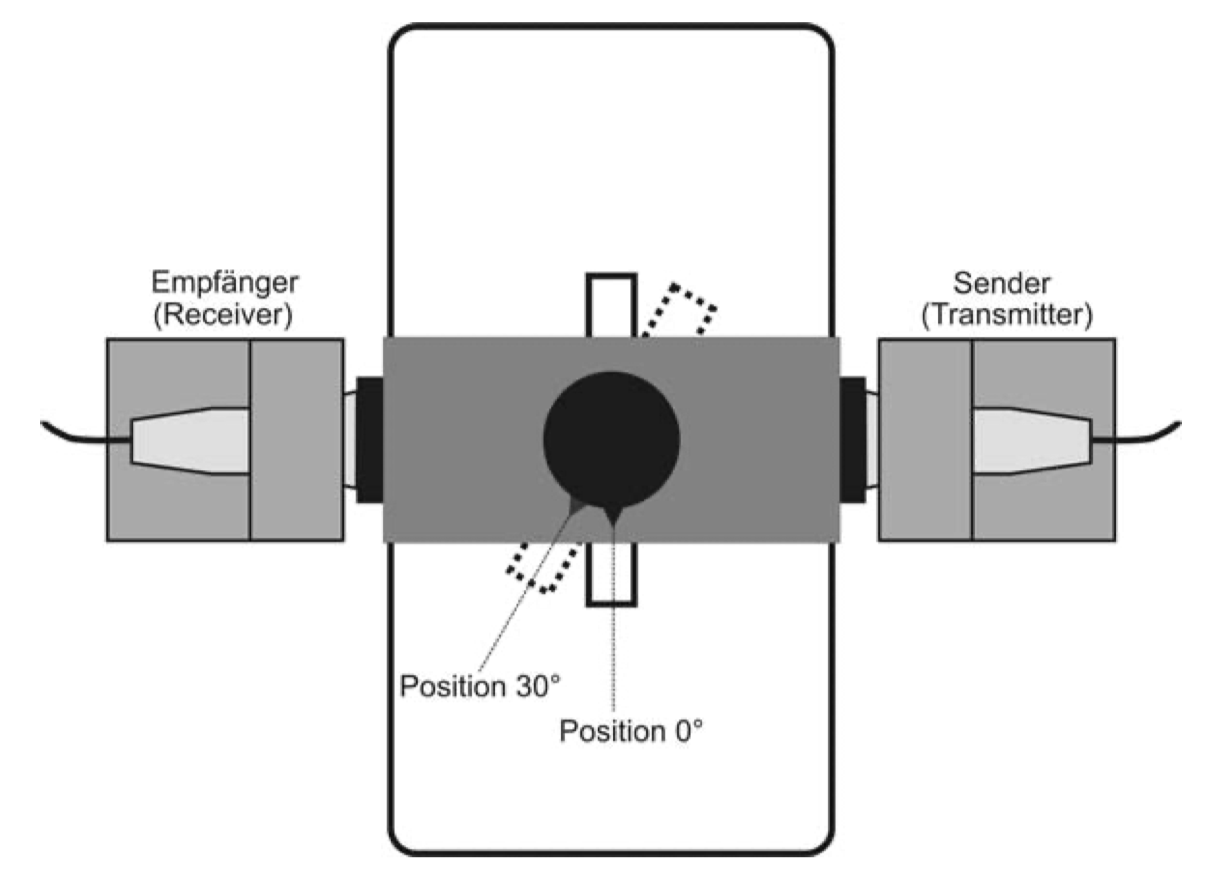
\includegraphics[width=0.5\textwidth]{PHY07_app.png}
    \caption{PHY07實驗器材架設示意圖}
    \label{fig:phy07app}
\end{figure}

\section{結果與討論}

不同入射角下的橫縱波之透射振幅如圖\ref{fig:07result}。
並利用訊號消失前的最後幾個點做線性迴歸得到斜率$a$與$y$截距$b$(帶有不確定度)。其$x$截距$-b/a$即為全反射角$\phi$。另外也可以直接由圖形得出橫波發生最大透射的角度$\Phi$。使用這些角度求出的波速如表\ref{tab:phy07_speed1},可以發現使用$\Phi$角計算的鋁的橫波波速結果不準確,這原因是因為我們對於入射角的調整不夠精細導致,這也導致鋁的各個測量值由於數據點少而不確定度更大。而其他的測量結果,雖然誤差較小,但也沒有包含在不確定度範圍內。注意到訊號在消失前還有一段翹起,這可能是因為聲波繞過板子兩側而被探針接收。這可能是波速的測量產生偏差的原因。由於其中聲場幾何形狀複雜,無法對此偏差進行定量分析。

\begin{figure}[htbp]
    \centering
    \begin{subfigure}{0.49\textwidth}
        \centering
        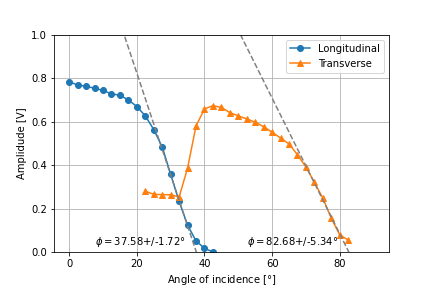
\includegraphics[width=\textwidth]{Acrylic.png}
        \caption{壓克力板}
        \label{fig:acrylic}
    \end{subfigure}
    \hfill
    \begin{subfigure}{0.49\textwidth}
        \centering
        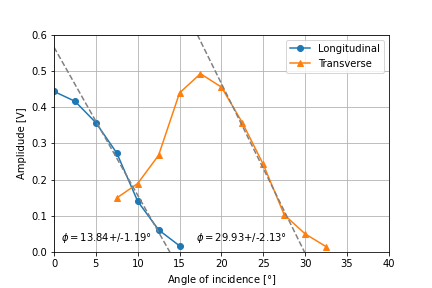
\includegraphics[width=\textwidth]{Aluminium.png}
        \caption{鋁}
        \label{fig:aluminium}
    \end{subfigure}
    \caption{不同入射角下的橫縱波之透射振幅}
    \label{fig:07result}
\end{figure}

\begin{table}[htbp]
    \centering
    \caption{使用全反射和橫波最大透射計算出的波速(單位:m/s)}
    \label{tab:phy07_speed1}
    \begin{tabular}{@{}llllll@{}}
    \toprule
              & $c_L=c_0/\sin\phi_L$ & $c_L$理論值  & $c_T=c_0/\sin\phi_T$ & $c_T=c_0/(\sqrt{2}\sin\Phi)$ & $c_T$理論值  \\ \midrule
    壓克力   & \SI{2.44(10)e3}{}    & 2610-2780 & \SI{1502(18)}{}      & \SI{1.56(4)e3}{}             & 1430-1450 \\
    鋁 & \SI{6.2(5)e3}{}      & 6320-6420 & \SI{2.99(19)e3}{}    & \SI{3.50(24)e3}{}            & 3040-3160 \\ \bottomrule
    \end{tabular}
    \vspace{5mm}
    \caption{材料的彈性係數的計算}
    \label{tab:elas}
    \begin{tabular}{@{}ccccccc@{}}
    \toprule
              & $\nu$          & 理論值  & $G$ [MPa]         & 理論值   & $E$ [MPa]         & 理論值   \\ \midrule
    壓克力   & \SI{0.20(4)}{} & 0.29 & \SI{2.71(6)e3}{}  & 2600  & \SI{6.48(23)e3}{} & 6800  \\
    鋁 & \SI{0.35(4)}{} & 0.31 & \SI{2.41(31)e4}{} & 26000 & \SI{6.5(7)e4}{}   & 68000 \\ \bottomrule
    \end{tabular}
\end{table}
由於$\Phi$得到的數據較為不準,接下來僅使用全反射的數據。將式\eqref{speed_ratio}改寫為
\begin{equation}
    \nu = \frac{2-(c_L/c_T)^2}{2-2(c_L/c_T)^2}
\end{equation}
可以求得$\nu$,並利用\eqref{speed1}和\eqref{speed2}可以求出$G,E$。在不確定度的範圍下大致準確,產生偏差的主要原因則是因為我們計算波速時的偏差。
紀錄於表\ref{tab:elas}中。

\chapter{PHY23 Dispersion of ultrasonic waves (Lamb waves)}\label{PHY23}

\section{實驗目的}

了解不同stimulated mode下的Lamb Wave群速度,並測量其隨頻率的變化並與理論圖形比較。

\section{實驗原理}

\subsection{Lamb Wave}

圖\ref{fig:lw}展示了Lamb wave傳播的示意圖,在薄板中
因為波速的不同使得橫波與縱波有不同的反射角。實驗中我們將會使用不同角度
的探針入射,激發出各種主要模態並計算其傳遞速率。
\begin{figure}[htbp]
    \centering
    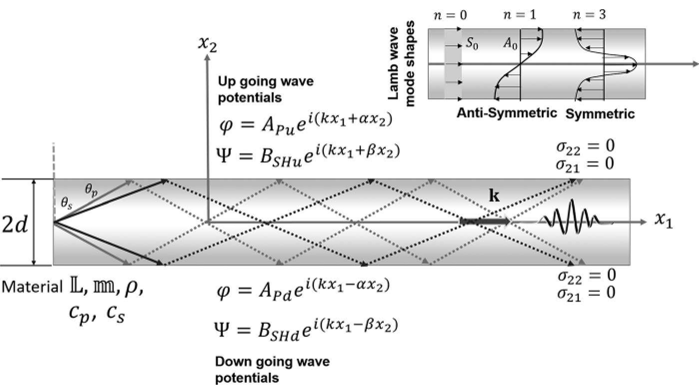
\includegraphics[width=0.6\textwidth]{lamb_wave_scheme.png}
    \caption{由橫波和縱波組成的Lamb Wave在兩個 Traction free 介面
    包圍形成的板狀結構示意圖。呈現對稱和反對稱波形}
    \label{fig:lw}
\end{figure}

\section{實驗步驟}

\begin{enumerate}
    \item 測量不同薄板的厚度。
    \item 選取不同頻率的兩個探針,連接探針並調整至 transmission mode。
    \item 選用不同的薄板厚度與不同角度的楔形套子,將探針、套子、薄板之間圖上傳導膠。

    \item 將薄板用膠帶固定在帶有刻度的的方格紙上,並再用膠帶固定一個塑膠尺在薄版上用來對齊探針的位置,將兩個探針的套子的頂點面對面擺放,如圖\ref{fig:f2f}。
    
    有時候我們可能會無法確認頂點是否對齊,這時可以透過轉動探針使得測到的訊號振幅最大,此時兩探針的頂點應該是對齊的。
    也能發現到在轉動探針時回聲的位置並不會有太大的影響。

    \item 將探針靠著直尺移動改變兩探針的距離,紀錄兩探針在不同距離$s$下與探針接收到的脈衝的峰值時間$t$,將$s$對$t$進行線性回歸得到群速度$v_{\rm g}$,並確認測量到群速度與理論群速度數值是否吻合。

    講義中僅使用探針靠在一起時測得的時間$t_0$,與拉開一段距離$s$後測得的時間$t$計算群速度$v_{\rm g}= 
    x_1/(t_1-t_0)$。紀錄更多的距離與時間可以使得結果更準確,且我們可以透過回歸直線來計算斜率的不確定度,也能用$R^2$值來驗證追蹤的波包由是同一個模態產生。
\end{enumerate}

\begin{figure}[htbp]
    \centering
    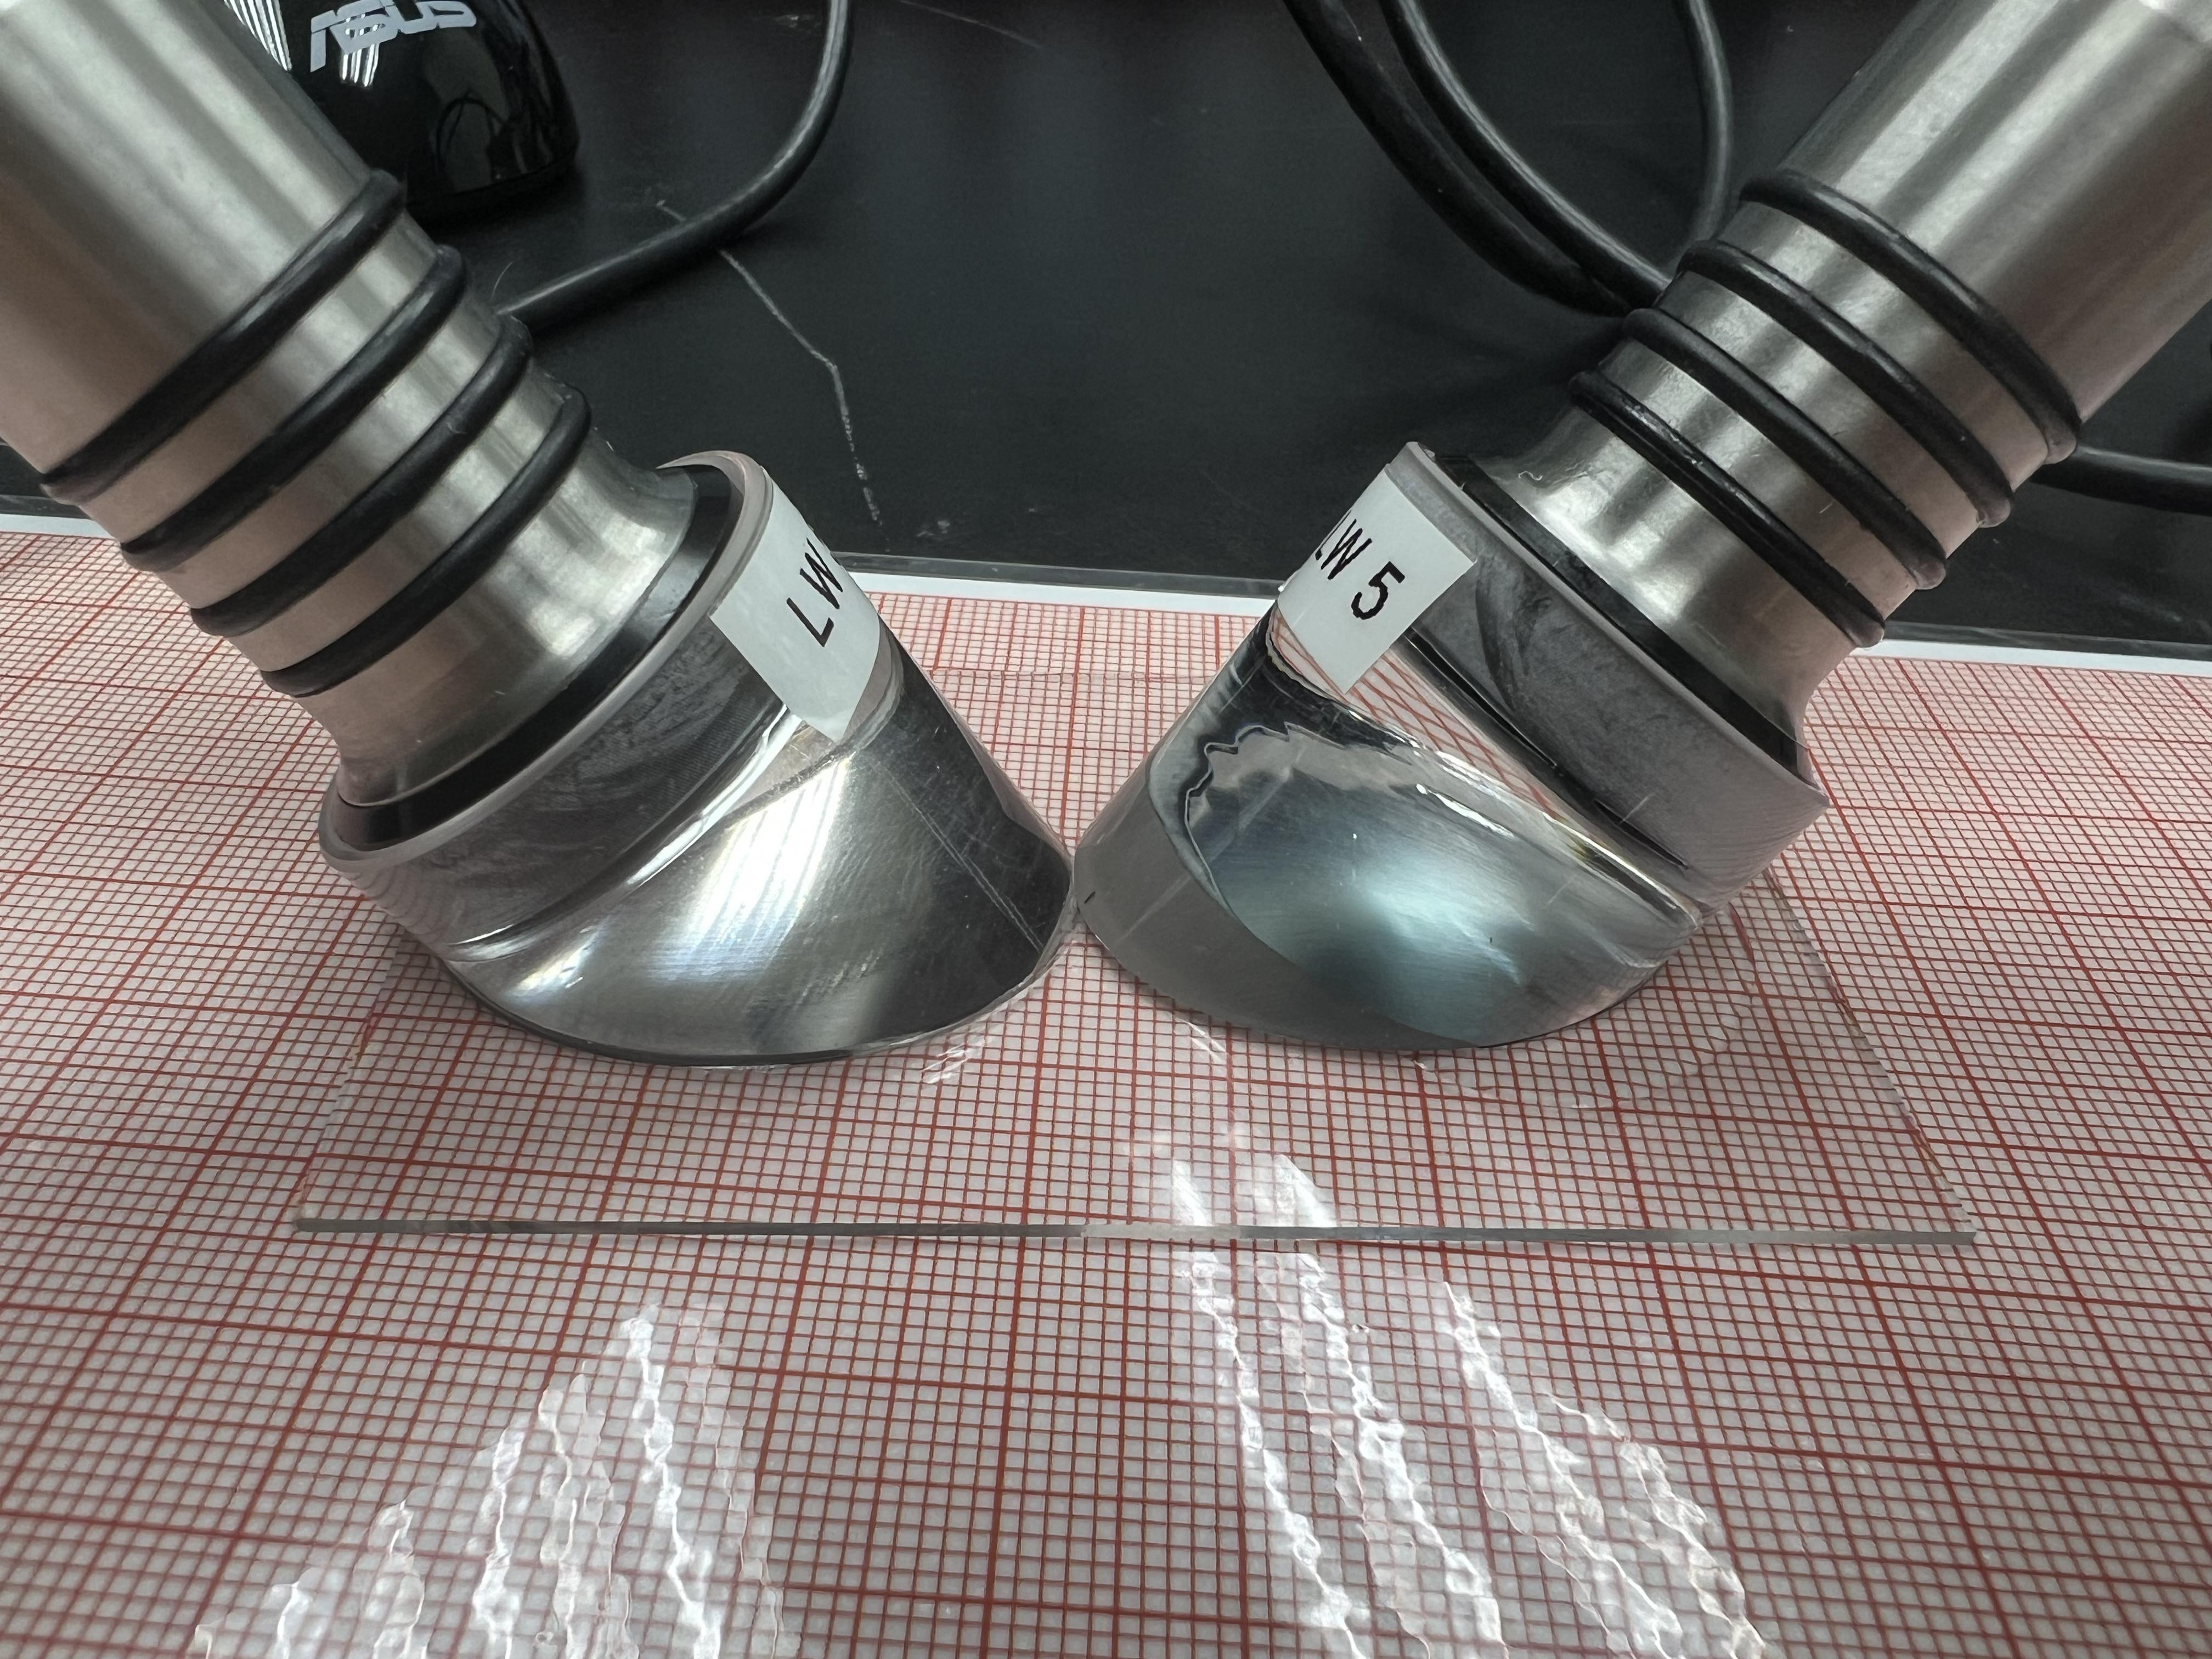
\includegraphics[width=0.6\textwidth]{f2f.jpeg}
    \caption{兩個探針收發的方式示意圖,圖中為楔形套子頂點靠在一起的情況}
    \label{fig:f2f}
\end{figure}
 
本實驗需測量的 mode 與對應的探針頻率如表\ref{tab:lwset}。表中列出了不同角度與厚度組合將激發出的主要模態,然而也會有幾個數個次要模態被激發,所以實際上的波形會是由數個模態混合形成,這也是為什麼我們只能讀取波包的峰值時間來計算群速度。為了準確的找出主要模態,我們先使用FFT計算薄板被激發出的實際頻率$f$,先計算理論的群速度數值作為基準值。

在使用2 MHz測量LW1的時候,發現主要受激的A1模態有時候會不明顯,例如當$s=\SI{3}{mm}$波形如圖\ref{fig:3mm},不同mode的振幅大小相近,且有互相混合的現象。當距離拉遠,不同模態的的群速度不同使得他們會逐漸分離開來,例如當$s=\SI{9}{mm}$的時候波形如圖\ref{fig:9mm},此時主要模態較為明顯且與次要模態分離開來。

在這個例子中還發現了可以透過FFT判斷主要模態是否明顯,將訊號進行FFT時會發現頻域上有數個峰,這些應該對應到被激發出的不同
模態的頻率,可以發現當時域上有一個較為明顯的的波包時,其中一個峰也會變得更明顯。找出了主要模態對應的峰之後,我們只在這個
峰足夠大的時候紀錄數據,避免因為不同模態混合造成的影響。


\begin{figure}[htbp]
    \centering
    \begin{subfigure}{0.49\textwidth}
        \centering
        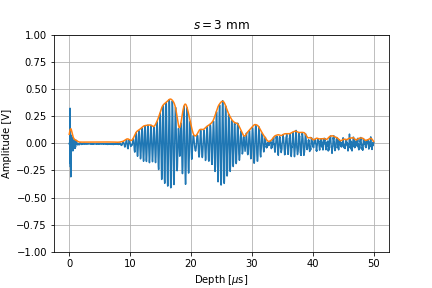
\includegraphics[width=\textwidth]{3.png}
        \caption{$s=\SI{3}{mm}$,此時沒有明顯主要模態}
        \label{fig:3mm}
    \end{subfigure}
    \hfill
    \begin{subfigure}{0.49\textwidth}
        \centering
        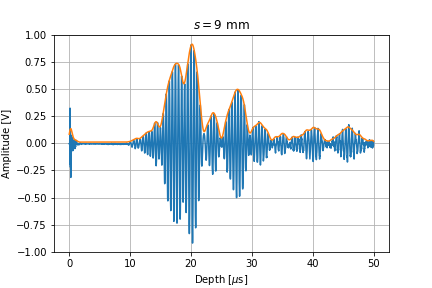
\includegraphics[width=\textwidth]{9.png}
        \caption{$s=\SI{9}{mm}$,此時A1主要模態顯現}
        \label{fig:9mm}
    \end{subfigure}
    \caption{2 MHz探針測量LW1的情況}
    \label{fig:2mhzlw1}
\end{figure}

\begin{table}[htbp]
\centering
\caption{本實驗使用的激發頻率與入射角組合與對應的主要受激模態}
\label{tab:lwset}
\begin{tabular}{@{}cccll@{}}
\toprule
\multicolumn{1}{l}{玻璃厚度$d$} & \multicolumn{1}{l}{}    & 入射角$\alpha_{\rm W}$                  & 激發頻率 & 模態 \\ \midrule
\multirow{8}{*}{1 mm}    & \multirow{2}{*}{LW1}    & \multirow{2}{*}{12°} & 2 MHz         & A1     \\
                         &                         &                      & 4 MHz         & S2     \\ \cmidrule(l){2-5} 
                         & \multicolumn{1}{l}{LW2} & 15°                  & 2 MHz         & A1     \\ \cmidrule(l){2-5} 
                         & \multirow{2}{*}{LW3}    & \multirow{2}{*}{28°} & 2 MHz         & S0     \\
                         &                         &                      & 4 MHz         & A1     \\ \cmidrule(l){2-5} 
                         & \multicolumn{1}{l}{LW4} & 32°                  & 4 MHz         & A1     \\ \cmidrule(l){2-5} 
                         & \multirow{2}{*}{LW5}    & \multirow{2}{*}{35°} & 1 MHz         & S0     \\
                         &                         &                      & 2 MHz         & S0     \\ \midrule
\multirow{3}{*}{1.3 mm}  & \multirow{2}{*}{LW6}    & \multirow{2}{*}{25°} & 1 MHz         & S0     \\
                         &                         &                      & 2 MHz         & A1     \\ \cmidrule(l){2-5} 
                         & \multicolumn{1}{l}{LW7} & 32°                  & 2 MHz         & S0     \\ \bottomrule
\end{tabular}
\end{table}

\section{結果與討論}

得到的數據如表\ref{tab:phy23},將群速度$v_{\rm g}$對頻率$f$乘以薄板厚度$d$作圖,如圖\ref{fig:phy21}。
得到的數據大致準確,測量值的不確定度範圍有包含理論值。但
其中還是有一些數據點有誤差,其產生原因可能同樣來自於不同模態混合
導致波包峰值位置的判讀有偏差,也有可能是FFT時因為選取的範圍不當使得求出的頻率有偏差,導致
測量值與錯誤的理論值做比較。

注意到使用前述的方法測量2 MHz、LW1的數據點的時候,因為主要模態明顯的距離很少,只有取三個點做群速度的擬合,所以
不確定度較大且$R^2$較小,但最後求出的最佳估計值與理論值的誤差非常小。

\begin{table}[htbp]
    \centering
    \caption{群速度的測量數據}
    \label{tab:phy23}
    \begin{tabular}{@{}llccccccr@{}}
    \toprule
    Mode                         & Set & $f$  & $d$  & $fd$ & $v_g$測量值    & $R^2$  & $v_g$理論值& 誤差     \\
                             &  & MHz & mm & MHz mm & km/s    &   & km/s &      \\ \midrule
    \multirow{5}{*}{${\rm S_0}$} & LW5 & 1.03    & 0.96   & 0.99      & \SI{5.51(11)}{} & 0.9973 & 5.431          & 1.5\%   \\
                                 & LW6 & 1.17    & 1.28   & 1.50      & \SI{4.81(11)}{} & 0.9964 & 5.241          & -8.2\%  \\
                                 & LW5 & 2.44    & 0.96   & 2.34      & \SI{3.91(9)}{} & 0.9960 & 3.095          & 26.4\%  \\
                                 & LW3 & 1.76    & 1.02   & 1.80      & \SI{5.50(8)}{} & 0.9986 & 4.956          & 11.0\%  \\
                                 & LW7 & 1.76    & 1.00   & 2.11       & \SI{5.35(5)}{} & 0.9994 & 4.307          & 24.2\%  \\ \midrule
    \multirow{5}{*}{${\rm A_1}$} & LW1 & 2.05    & 1.00      & 2.05        & \SI{2.8(5)}{}   & 0.9712 & 2.784          & 0.6\%   \\
                                 & LW2 & 2.15    & 1.00   & 2.15        & \SI{3.02(9)}{} & 0.9938 & 3.099          & -2.6\%  \\
                                 & LW6 & 2.34    & 1.28   & 3.00      & \SI{4.27(8)}{} & 0.9985 & 3.984          & 7.2\%   \\
                                 & LW3 & 3.72    & 1.02   & 3.79      & \SI{3.23(10)}{} & 0.9887 & 3.729          & -13.4\% \\
                                 & LW4 & 4.39    & 1.00   & 4.39        & \SI{2.84(15)}{} & 0.9949 & 2.980          & -4.7\%  \\ \midrule
    ${\rm S_2}$                  & LW1 & 4.10     & 1.00   & 4.10        & \SI{2.76(14)}{}  & 0.9916 & 2.845          & -2.9\%  \\ \bottomrule
    \end{tabular}
\end{table}

\begin{figure}[htbp]
    \centering
    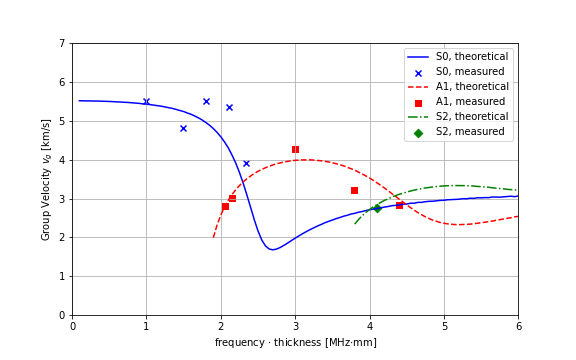
\includegraphics[width=0.8\textwidth]{PHY21.png}
    \caption{Lame wave 的S0, A1, S2模態的群速度測量結果與理論曲線}
    \label{fig:phy21}
\end{figure}






\chapter{PHY11 Debye-Sear effect}\label{PHY11}

\section{實驗目的}
利用超聲波在透明液體(本實驗採用去離子水)中形成的駐波對雷射光進行干涉,以此來計算超聲波在液體中的波長與聲速。
\section{實驗原理}
Debye–Sears效應是在描述超聲波在液體中所形成的駐波能作為光柵對雷射光進行干涉的現象。實驗中我們將發送固定頻率$f$之超聲波至水中,並量測干涉條紋的最大級數 $N$、水平投影距離 $s$,以及$+N$至$-N$級數之干涉條紋之間的距離$x$,即可以用雷射光之波長$\lambda_L$求得超聲波在液體中的波長$\lambda_S$與聲速$c$。
\begin{equation}
    \lambda_S=2N\cdot\lambda_L\frac{s}{x}
\end{equation}
\begin{equation}
    c=\lambda_S\cdot f
\end{equation}
\begin{figure}
    \centering
    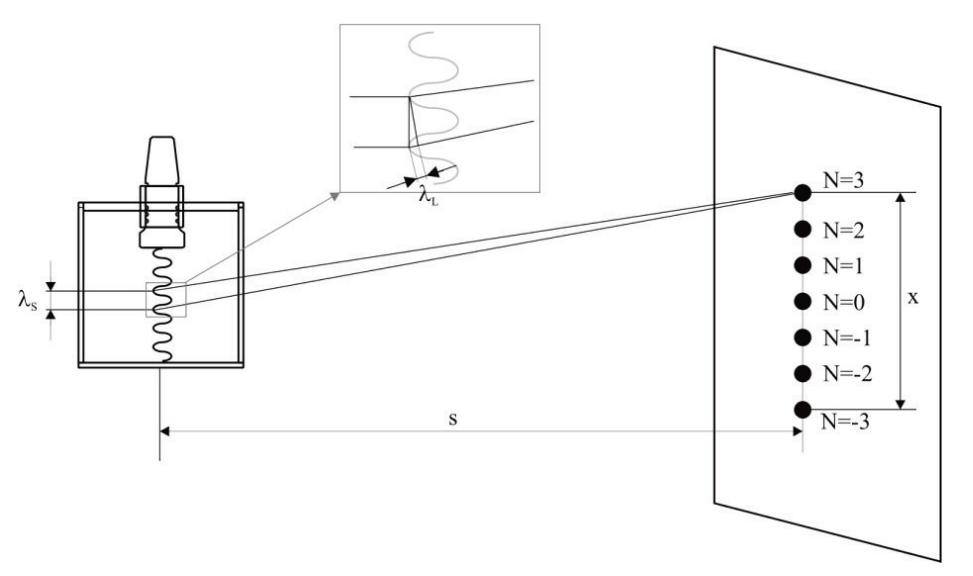
\includegraphics[width=0.5\linewidth]{PHY11-1.png}
    \caption{Debye–Sears效應示意圖}
    \label{fig:PHY11_1}
\end{figure}
\section{實驗步驟}
\begin{enumerate}
    \item 將Debye-Sears set中的容器注入去離子水,並將可變頻率的Probe與綠光雷射分別接到容器蓋與容器側壁中。
    \item 將Probe與雷射接至SC600 sound wave controller上。
    \item 開啟雷射並調整其功率,並移動容器使通過液體的雷射可以打到實驗桌旁架子上的反射鏡,再由反射鏡打到牆壁上。
    \item 透過微調容器蓋上的旋鈕,調整光路。
    \item 測量Probe至反射鏡以及反射鏡至牆壁雷射光點處的距離,並計算總距離$s$。
    \item 按下SC600 sound wave controller上Probe的開關。調整Frequency Generator使Probe的頻率至$\SI{1}{MHz}$。調整Probe的功率使干涉條紋出現。
    \item \label{Nx}測量兩兩干涉條紋之間的距離$x_0$;干涉條紋的最大級數$N$,以及$+N$至$N$級數之干涉條紋之間的距離$x$。
    \item \label{fre}調整Frequency Generator,使Probe的頻率增加$\SI{1}{MHz}$。重複步驟\ref{Nx} 與\ref{fre} 直到$N\neq 0$階的干涉條紋難以判讀。
    \item 將雷射換成紅光雷射,並重複以上步驟。
    
\end{enumerate}
\subsection*{觀察}
\begin{itemize}
    \item 要注意將容器注入去離子水時,水位應恰好覆蓋過Probe的頭,才能有效的在水中產生超聲波。
    \item 在計算總距離$s$時,要注意測量必須從Probe開始。這是因為繞射是從Probe開始的,我們可以從圖\ref{fig:PHY11_1}中看出這一點。
    \item 在測量$+N$至$-N$級數之干涉條紋之間的距離$x$時,要確定干涉峰為奇數($1+2N$)個,才能正確得測量$x$。
    \item 在步驟\ref{Nx} 中之所以要額外測量兩兩干涉條紋之間距$x_0$,是為了要確保干涉條紋的最大級數$N$沒有判讀錯誤。我們可以使用關係式$N=x/2x_0$來驗證所測得的$N$。然而因為$x_0$很小,所求出的$N$誤差很大,僅能粗略地驗證是否判讀出錯誤的$N$,我們將在結果中看到這一點。
    
\end{itemize}
\section{結果與討論}
$x$是由游標尺測量,游標尺最小單位\SI{0.02}{mm},因此會有B類不確定度為$\SI{0.02}{mm}/\sqrt{3}=\SI{0.01}{mm}$。而$s$則是由捲尺測量,尺最小單位\SI{0.1}{cm},因此會有B類不確定度為$\SI{0.1}{cm}/\sqrt{3}=\SI{0.05}{cm}$。然而,我們認為由於Probe的直徑會造成繞射位置的不確定,而對總長$s$造成一不確定度。取其直徑約為 \SI{2}{cm},以B類不確定度的取法得到其會造成\SI{1}{cm}的不確定度。

表\ref{table:green}和表\ref{table:red}中列出了所測量出的$x$、$x_0$、$N$,以及計算出的$\lambda_S$與$c$。其中$x_0$與$x/2x_0$項只是為了協助判讀$N$,故不計算不確定度。

\begin{table}[htbp]
\centering
\caption{綠光雷射的實驗數據,其中$\lambda_L=\SI{532}{nm}$、$s=\SI{285(1)}{cm}$。}
\begin{tabular}{ccccccc}
\hline
$f$ (MHz) & $N$ & $x_0$ (mm) & $x$ (mm) & $x/2x_0$ & $\lambda_S$($\si{\mu m}$) & $c$(m/s) \\ \hline
1  & 11 & 1.0 & \SI{22.30(1)}{} & 11.15 & \SI{1501(5)}{} & \SI{1501(5)}{}\\ \hline
2  & 3  & 2.1 & \SI{12.48(1)}{} & 2.971 & \SI{731(3)}{}  & \SI{1463(6)}{}\\ \hline
3  & 6  & 3.5 & \SI{36.78(1)}{} & 5.254 & \SI{496(2)}{}  & \SI{1489(6)}{}\\ \hline
4  & 4  & 4.5 & \SI{32.46(1)}{} & 3.607 & \SI{375(1)}{}  & \SI{1500(4)}{}\\ \hline
5  & 4  & 5.5 & \SI{41.84(1)}{} & 3.804 & \SI{291(1)}{}  & \SI{1454(5)}{}\\ \hline
6  & 4  & 5.9 & \SI{48.80(1)}{} & 4.136 & \SI{250(1)}{}  & \SI{1496(6)}{}\\ \hline
7  & 3  & 7.3 & \SI{43.20(1)}{} & 2.959 & \SI{211(1)}{}  & \SI{1479(7)}{}\\ \hline
8  & 1  & 8.0 & \SI{16.44(1)}{} & 1.028 & \SI{185(1)}{}  & \SI{1481(8)}{}\\ \hline
9  & 1  & 8.8 & \SI{18.24(1)}{} & 1.036 & \SI{167(1)}{}  & \SI{1501(9)}{}\\ \hline
10 & 1  & 9.9 & \SI{20.98(1)}{} & 1.060 & \SI{145(1)}{}  & \SI{1450(10)}{}\\ \hline
   &    &     &          &       & mean    & \SI{1481(2)}{}   \\
   &    &     &          &       & SD      & 20     \\
\end{tabular}
\label{table:green}
\end{table}

\begin{table}[htbp]
\centering
\caption{紅光雷射的實驗數據,其中$\lambda_L=\SI{650}{nm}$、$s=\SI{285(1)}{cm}$。}
\begin{tabular}{ccccccc}
\hline
$f$ (MHz) & $N$ & $x_0$ (mm) & $x$ (mm) & $x/2x_0$ & $\lambda_S$($\si{\mu m}$) & $c$(m/s) \\ \hline
1  & 12 & 1.2  & \SI{28.94(1)}{} & 12.06 & \SI{1541(5)}{} &\SI{1541(5)}{} \\ \hline
2  & 3  & 3.0  & \SI{15.36(1)}{} & 2.56  & \SI{726(3)}{}  &\SI{1452(6)}{}  \\ \hline
3  & 4  & 4.2  & \SI{29.98(1)}{} & 3.57  & \SI{496(2)}{}  &\SI{1488(6)}{}  \\ \hline
4  & 5  & 5.1  & \SI{50.00(1)}{} & 4.90  & \SI{372(1)}{}  &\SI{1488(4)}{}  \\ \hline
5  & 4  & 5.2  & \SI{49.90(1)}{} & 4.80  & \SI{298(1)}{}  &\SI{1490(5)}{}  \\ \hline
6  & 4  & 7.5  & \SI{60.00(1)}{} & 4.00  & \SI{248(1)}{}  &\SI{1488(6)}{}  \\ \hline
7  & 3  & 8.6  & \SI{52.74(1)}{} & 3.07  & \SI{212(1)}{}  &\SI{1477(7)}{}  \\ \hline
8  & 2  & 10.0 & \SI{39.66(1)}{} & 1.98  & \SI{188(1)}{}  &\SI{1496(8)}{}  \\ \hline
9  & 1  & 10.9 & \SI{22.98(1)}{} & 1.05  & \SI{162(1)}{}  &\SI{1458(9)}{}  \\ \hline
   &    &     &          &       & mean    & \SI{1486(2)}{}   \\
   &    &     &          &       & SD      & 25     \\
\end{tabular}
\label{table:red}
\end{table}












\chapter{回答問題}

本次實驗的手冊沒有提供問題,我們在這裡嘗試推導前述實驗中的理論模型

\section{吸收導致的聲波衰減}

在PHY04提到聲波在液體中傳播時,由於吸收(能量轉換)、反射、散射或聲場的幾何形狀而衰減。在這裡說明吸收所導致的聲波衰減為指數遞減的形式。這些吸收會將聲波的力學能轉變為其他能量,由一個 relaxation time $\tau$所描述。考慮帶有 relaxation terms 的聲波方程\footnote{Kinsler, L.E., Frey, A.R., Coppens, A.B. and Sanders, J.V. (2000) Fundamentals of Acoustics. 4th Edition, John Wiley and Sons Inc., Hoboken.}
\begin{equation}
    \nabla^2 p - \frac{1}{c^2} \pdv[2]{p}{t} =-\tau\pdv{t}(\nabla^2 p)
\end{equation}
考慮以下形式的(複數)解
\begin{equation}
    p(x,t)=A e^{i(\omega t -kx)}
\end{equation}
可以解得
\begin{equation}
    k=k_r-i\frac{\alpha}{2}=\frac{\omega}{c\sqrt{1+i\omega\tau}}
\end{equation}
所以聲場在空間中有為指數衰減的形式
\begin{equation}
    p(x,t)=Ae^{-\alpha x/2}e^{i(\omega t - k_r x)}
\end{equation}
且由於聲強$I\propto \langle p^2 \rangle$,所以
\begin{equation}
    I(x)=I_0 e^{-\alpha x}
\end{equation}

\section{斜入射的透射與反射}

\begin{figure}[htbp]
    \centering
    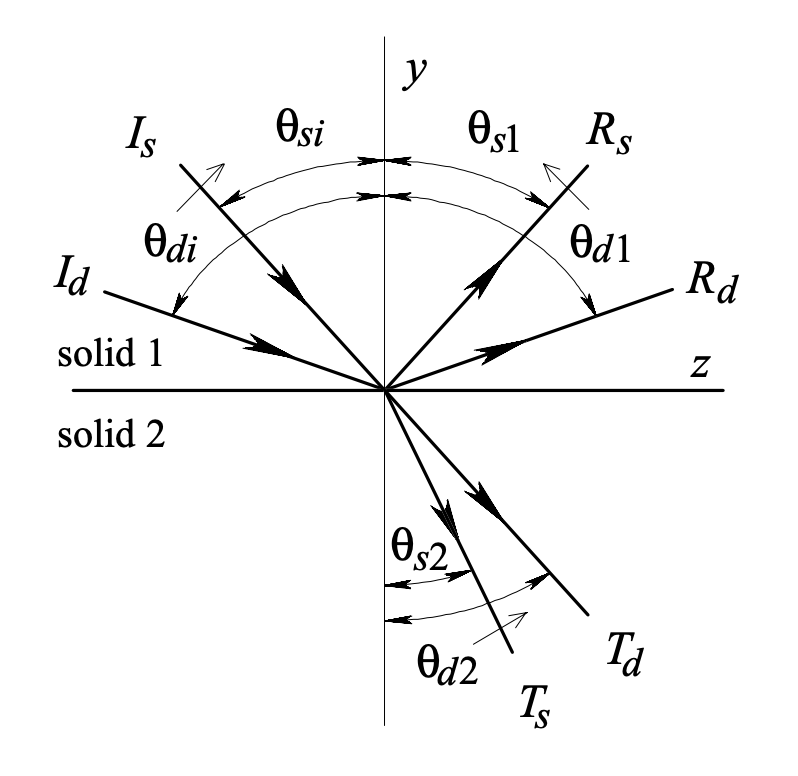
\includegraphics[width=0.5\textwidth]{oblique.png}
    \caption{固體、固體介面之間的斜入射}
    \label{oblique}
\end{figure}

考慮最廣義的情況:聲波從固體入射固體,如圖\ref{oblique}\footnote{B. A.
Auld Acoustic Fields and Waves (John Wiley \& Sons, New York, 1973) Vol. II, pp. 21-38.}。當入射波(含有橫波和縱波的成分)以斜角入射時,將會反射與折射出橫波(transverse; shear)與縱波(longitudinal; dilational),這些角度滿足Snell's law
\begin{equation}
    \frac{\sin\theta_{di}}{c_{di}}
    =\frac{\sin\theta_{si}}{c_{si}}
    =\frac{\sin\theta_{d1}}{c_{d1}}
    =\frac{\sin\theta_{s1}}{c_{s1}}
    =\frac{\sin\theta_{d2}}{c_{d2}}
    =\frac{\sin\theta_{s2}}{c_{s3}}
\end{equation}
入射、反射、透射的粒子位移的振幅分別記為$I,R,T$,以下標區分橫波與縱波。兩介面之間的邊界條件要求$u_y, u_z$與這兩個stress components的連續性
\begin{equation}
    \tau_{yy}=\lambda\pdv{u_z}{z}+(\lambda+2\mu)\pdv{u_y}{y}
\end{equation}
和
\begin{equation}
    \tau_{zy}=\mu\left(\pdv{u_y}{z}+\pdv{u_z}{y}\right)
\end{equation}
其中$\mu=\rho c_{s}^2, \lambda+2\mu=\rho c_{d}^2$。所以有
\begin{equation}
    \left[\begin{array}{l}
        u_y^{(2)}-u_y^{(1)} \\
        u_z^{(2)}-u_z^{(1)} \\
        \tau_{y y}^{(2)}-\tau_{y y}^{(1)} \\
        \tau_{z y}^{(2)}-\tau_{z y}^{(1)}
        \end{array}\right]=\left[\begin{array}{l}
        0 \\
        0 \\
        0 \\
        0
        \end{array}\right] \text { or }\left[\begin{array}{l}
        -u_y^{(d 1)}+u_y^{(d 2)}-u_y^{(s 1)}+u_y^{(s 2)} \\
        -u_z^{(d 1)}+u_z^{(d 2)}-u_z^{(s 1)}+u_z^{(s 2)} \\
        -\tau_{y y}^{(d 1)}+\tau_{y y}^{(d 2)}-\tau_{y y}^{(s 1)}+\tau_{y y}^{(s 2)} \\
        -\tau_{z y}^{(d 1)}+\tau_{z y}^{(d 2)}-\tau_{z y}^{(s 1)}+\tau_{z y}^{(s 2)}
        \end{array}\right]=\left[\begin{array}{c}
        u_y^{(i)} \\
        u_z^{(i)} \\
        \tau_{y y}^{(i)} \\
        \tau_{z y}^{(i)}
        \end{array}\right]
\end{equation}
其中我們可以區分縱波入射($I_d=1, I_s=0$)與橫波入射($I_s=1, I_d=0$),可以將其寫成矩陣形式$\mathsf{A} \vb{x}=\vb{b}$,其中$x=[R_d\ T_d\ R_s\ T_s]^T$,矩陣為
\begin{equation}
    \mathsf{A}=\left[\begin{array}{cccc}
        -\cos \theta_{d 1} & -\cos \theta_{d 2} & -\sin \theta_{s 1} & \sin \theta_{s 2} \\
        -\sin \theta_{d 1} & \sin \theta_{d 2} & \cos \theta_{s 1} & \cos \theta_{s 2} \\
        -Z_{d 1} \cos 2 \theta_{s 1} & Z_{d 2} \cos 2 \theta_{s 2} & -Z_{s 1} \sin 2 \theta_{s 1} & -Z_{s 2} \sin 2 \theta_{s 2} \\
        -Z_{s 1} \frac{c_{s 1}}{c_{d 1}} \sin 2 \theta_{d 1} & -Z_{s 2} \frac{c_{s 2}}{c_{d 2}} \sin 2 \theta_{d 2} & Z_{s 1} \cos 2 \theta_{s 1} & -Z_{s 2} \cos 2 \theta_{s 2}
        \end{array}\right]
\end{equation}
而$\vb{b}$的形式取決於縱波或橫波入射
\begin{equation}
    b=\left[\begin{matrix}-\cos\theta_{di}\\\sin\theta_{di}\\Z_{d1}\cos 2\theta_{si}\\-Z_{s1}\frac{c_{s1}}{c_{d1}}\sin 2\theta_{di}\end{matrix}\right] \text{ or }
        \left[\begin{matrix}\sin\theta_{si}\\\cos\theta_{si}\\-Z_{s1}\sin 2\theta_{si}\\-Z_{s1}\cos 2\theta_{si}\end{matrix}\right] 
\end{equation}
透過對這個線性方程組求解,可以得到不同入射角$\theta_i$的反射率和透射率。

在PHY07實驗中,為液體入射固體的情況,所以是縱波入射的情況,且沒有反射的橫波。線性方程組變為    
    \begin{equation}
    a = \left[\begin{matrix}
    -\cos\theta  &  -\cos\theta_L  &  \sin\theta_T \\
    -\sin\theta  &  \sin\theta_L  &  \cos\theta_T \\
    0  &  \frac{c_T}{c_L}\sin 2\theta_L  &  \cos 2\theta_T
    \end{matrix}\right]
    \left[\begin{matrix}R_d\\T_d\\T_s\end{matrix}\right]
    =\left[\begin{matrix}-\cos\theta\\\sin\theta\\0\end{matrix}\right]
    \end{equation}
其中\begin{equation}
    \frac{\sin\theta}{c_0} = \frac{\sin\theta_L}{c_L} = \frac{\sin\theta_T}{c_T}
    \end{equation}
代入水的聲速和鋁的橫縱波聲速,使用python求解不同入射角$\theta$下此方程組的解,可以得到圖\ref{sim},雖然圖形和圖\ref{fig:aluminium}有所出入,但都可以發現在約\SI{13}{\degree}有一個臨界角。
\begin{figure}[htbp]
    \centering
    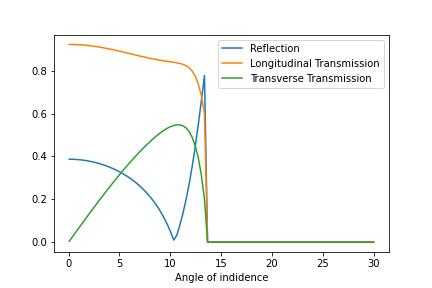
\includegraphics[width=0.5\textwidth]{sim.png}
    \caption{鋁浸沒與水中的反射與透射係數理論模型結果}
    \label{sim}
\end{figure}

\section{Lamb Wave的理論群速度}

接續節\ref{sec:wave_eqn}原理的討論,考慮一個厚度為$2h$的無限大薄板在$z=\pm h$之間。設$\phi=\phi(x,z), \vb\psi=(0,-\psi_y(x,z),0)$
並考慮以下形式的解
\begin{align}
    \phi&=\Lambda(z)e^{i(kx-\omega t)} \\
    \psi_y&=\Omega(z)e^{i(kx-\omega t)}
\end{align}
更進一步,區分對稱和反對稱的mode為:
\begin{align}
    \text{S mode: } & \Lambda(z)=A\cos(\alpha z),\quad \Theta(z)=B\sin(\beta z) \\
    \text{A mode: } & \Lambda(z)=A\sin(\alpha z),\quad \Theta(z)=B\cos(\beta z) \\
\end{align}
其中
\begin{align}
    \alpha^2&=\left(\frac{\omega}{c_L}\right)^2-k^2 \\
    \beta^2&=\left(\frac{\omega}{c_T}\right)^2-k^2 
\end{align}
代入邊界條件,可以得到Rayleigh-Lamb方程
\begin{equation}
    \frac{\tan(\beta h)}{\tan(\alpha h)}=\left[ 
    \frac{4k^2\alpha\beta}{(k^2-\beta^2)^2}
    \right]^{\pm 1}
\end{equation}
其中$\pm 1$分別對應到S/A mode。這是一個$\alpha$與$\beta$的隱函數,透過數值方法可以求出色散關係$\omega=\omega(k)$並求得相速度$v_{\rm p}=\omega/k$並進一步求得理論群速度$v_{\rm g}$:
\begin{equation}
    v_{\rm g} = \frac{c_{\rm p}^2}{c_{\rm p}-f\frac{dc_{\rm p}}{df}}
\end{equation}

\chapter{結論}

A5實驗的儀器操作較簡單,重點在於處理軟體獲得的數據從中獲取物理意義。

在PHY04實驗中我們了解了超聲波在介質中衰減的現象,需要綜合考量儀器處理訊號的過程,最終測得了水在室溫下的衰減係數$\alpha=\SI{1.493(32)}{dB/cm}$,雖然我們的模型擬合得很好,但結果還是有很大的正偏差,且我們只能給出定性的解釋,但能夠初步排除鋁板的部分反射造成的影響。比較可惜是我們們有分析衰減與聲波頻率的關係以及測量不同介質的衰減係數。在報告的最後我們嘗試定量推導聲波衰減的理論。

在PHY05實驗中我們透過超聲波在樣品內部來回反射導致的時間差計算樣品厚度,透過反射波的時間差推測超聲波在樣品內的行徑路線,並分別計算了A-scan、Spectrum、Cepstrum的峰值差來求得樣品厚度,並比較了不同方法的準確度與其原因。

在PHY06實驗中,我們使用不同頻率的超聲波測量兩孔洞之間的距離,發現了頻率較高的探針的聲波穿透力較差,且驗證了頻率越低的探針解析度越好。最後定性地計算脈衝寬度與波長之間的關係。

在PHY07和PHY23實驗中我們研究了固體樣品內產生的橫波與縱波,並研究了其透射率,利用全反射和尋找橫波最大透射兩種方式求出固體樣品的橫縱波聲速,並用於計算其彈性係數。在PHY23中則是研究了在薄板樣品中橫波與縱波混合產生出的不同模態的 Lame Wave,並測量其群速度與理論值比較。

在PHY11實驗中,我們驗證超聲波在水中傳遞對水分子的壓縮可以產生類似光閘的效果,並依此計算超聲波聲速和波長。


\bibliographystyle{unsrt} % We choose the "plain" reference style
\bibliography{ref.bib} % Entries are in the refs.bib file

\end{document}